% Options for packages loaded elsewhere
% Options for packages loaded elsewhere
\PassOptionsToPackage{unicode}{hyperref}
\PassOptionsToPackage{hyphens}{url}
\PassOptionsToPackage{dvipsnames,svgnames,x11names}{xcolor}
%
\documentclass[
  danish,
]{article}
\usepackage{xcolor}
\usepackage{amsmath,amssymb}
\setcounter{secnumdepth}{3}
\usepackage{iftex}
\ifPDFTeX
  \usepackage[T1]{fontenc}
  \usepackage[utf8]{inputenc}
  \usepackage{textcomp} % provide euro and other symbols
\else % if luatex or xetex
  \usepackage{unicode-math} % this also loads fontspec
  \defaultfontfeatures{Scale=MatchLowercase}
  \defaultfontfeatures[\rmfamily]{Ligatures=TeX,Scale=1}
\fi
\usepackage{lmodern}
\ifPDFTeX\else
  % xetex/luatex font selection
\fi
% Use upquote if available, for straight quotes in verbatim environments
\IfFileExists{upquote.sty}{\usepackage{upquote}}{}
\IfFileExists{microtype.sty}{% use microtype if available
  \usepackage[]{microtype}
  \UseMicrotypeSet[protrusion]{basicmath} % disable protrusion for tt fonts
}{}
\makeatletter
\@ifundefined{KOMAClassName}{% if non-KOMA class
  \IfFileExists{parskip.sty}{%
    \usepackage{parskip}
  }{% else
    \setlength{\parindent}{0pt}
    \setlength{\parskip}{6pt plus 2pt minus 1pt}}
}{% if KOMA class
  \KOMAoptions{parskip=half}}
\makeatother
% Make \paragraph and \subparagraph free-standing
\makeatletter
\ifx\paragraph\undefined\else
  \let\oldparagraph\paragraph
  \renewcommand{\paragraph}{
    \@ifstar
      \xxxParagraphStar
      \xxxParagraphNoStar
  }
  \newcommand{\xxxParagraphStar}[1]{\oldparagraph*{#1}\mbox{}}
  \newcommand{\xxxParagraphNoStar}[1]{\oldparagraph{#1}\mbox{}}
\fi
\ifx\subparagraph\undefined\else
  \let\oldsubparagraph\subparagraph
  \renewcommand{\subparagraph}{
    \@ifstar
      \xxxSubParagraphStar
      \xxxSubParagraphNoStar
  }
  \newcommand{\xxxSubParagraphStar}[1]{\oldsubparagraph*{#1}\mbox{}}
  \newcommand{\xxxSubParagraphNoStar}[1]{\oldsubparagraph{#1}\mbox{}}
\fi
\makeatother

\usepackage{color}
\usepackage{fancyvrb}
\newcommand{\VerbBar}{|}
\newcommand{\VERB}{\Verb[commandchars=\\\{\}]}
\DefineVerbatimEnvironment{Highlighting}{Verbatim}{commandchars=\\\{\}}
% Add ',fontsize=\small' for more characters per line
\usepackage{framed}
\definecolor{shadecolor}{RGB}{241,243,245}
\newenvironment{Shaded}{\begin{snugshade}}{\end{snugshade}}
\newcommand{\AlertTok}[1]{\textcolor[rgb]{0.68,0.00,0.00}{#1}}
\newcommand{\AnnotationTok}[1]{\textcolor[rgb]{0.37,0.37,0.37}{#1}}
\newcommand{\AttributeTok}[1]{\textcolor[rgb]{0.40,0.45,0.13}{#1}}
\newcommand{\BaseNTok}[1]{\textcolor[rgb]{0.68,0.00,0.00}{#1}}
\newcommand{\BuiltInTok}[1]{\textcolor[rgb]{0.00,0.23,0.31}{#1}}
\newcommand{\CharTok}[1]{\textcolor[rgb]{0.13,0.47,0.30}{#1}}
\newcommand{\CommentTok}[1]{\textcolor[rgb]{0.37,0.37,0.37}{#1}}
\newcommand{\CommentVarTok}[1]{\textcolor[rgb]{0.37,0.37,0.37}{\textit{#1}}}
\newcommand{\ConstantTok}[1]{\textcolor[rgb]{0.56,0.35,0.01}{#1}}
\newcommand{\ControlFlowTok}[1]{\textcolor[rgb]{0.00,0.23,0.31}{\textbf{#1}}}
\newcommand{\DataTypeTok}[1]{\textcolor[rgb]{0.68,0.00,0.00}{#1}}
\newcommand{\DecValTok}[1]{\textcolor[rgb]{0.68,0.00,0.00}{#1}}
\newcommand{\DocumentationTok}[1]{\textcolor[rgb]{0.37,0.37,0.37}{\textit{#1}}}
\newcommand{\ErrorTok}[1]{\textcolor[rgb]{0.68,0.00,0.00}{#1}}
\newcommand{\ExtensionTok}[1]{\textcolor[rgb]{0.00,0.23,0.31}{#1}}
\newcommand{\FloatTok}[1]{\textcolor[rgb]{0.68,0.00,0.00}{#1}}
\newcommand{\FunctionTok}[1]{\textcolor[rgb]{0.28,0.35,0.67}{#1}}
\newcommand{\ImportTok}[1]{\textcolor[rgb]{0.00,0.46,0.62}{#1}}
\newcommand{\InformationTok}[1]{\textcolor[rgb]{0.37,0.37,0.37}{#1}}
\newcommand{\KeywordTok}[1]{\textcolor[rgb]{0.00,0.23,0.31}{\textbf{#1}}}
\newcommand{\NormalTok}[1]{\textcolor[rgb]{0.00,0.23,0.31}{#1}}
\newcommand{\OperatorTok}[1]{\textcolor[rgb]{0.37,0.37,0.37}{#1}}
\newcommand{\OtherTok}[1]{\textcolor[rgb]{0.00,0.23,0.31}{#1}}
\newcommand{\PreprocessorTok}[1]{\textcolor[rgb]{0.68,0.00,0.00}{#1}}
\newcommand{\RegionMarkerTok}[1]{\textcolor[rgb]{0.00,0.23,0.31}{#1}}
\newcommand{\SpecialCharTok}[1]{\textcolor[rgb]{0.37,0.37,0.37}{#1}}
\newcommand{\SpecialStringTok}[1]{\textcolor[rgb]{0.13,0.47,0.30}{#1}}
\newcommand{\StringTok}[1]{\textcolor[rgb]{0.13,0.47,0.30}{#1}}
\newcommand{\VariableTok}[1]{\textcolor[rgb]{0.07,0.07,0.07}{#1}}
\newcommand{\VerbatimStringTok}[1]{\textcolor[rgb]{0.13,0.47,0.30}{#1}}
\newcommand{\WarningTok}[1]{\textcolor[rgb]{0.37,0.37,0.37}{\textit{#1}}}

\usepackage{longtable,booktabs,array}
\usepackage{calc} % for calculating minipage widths
% Correct order of tables after \paragraph or \subparagraph
\usepackage{etoolbox}
\makeatletter
\patchcmd\longtable{\par}{\if@noskipsec\mbox{}\fi\par}{}{}
\makeatother
% Allow footnotes in longtable head/foot
\IfFileExists{footnotehyper.sty}{\usepackage{footnotehyper}}{\usepackage{footnote}}
\makesavenoteenv{longtable}
\usepackage{graphicx}
\makeatletter
\newsavebox\pandoc@box
\newcommand*\pandocbounded[1]{% scales image to fit in text height/width
  \sbox\pandoc@box{#1}%
  \Gscale@div\@tempa{\textheight}{\dimexpr\ht\pandoc@box+\dp\pandoc@box\relax}%
  \Gscale@div\@tempb{\linewidth}{\wd\pandoc@box}%
  \ifdim\@tempb\p@<\@tempa\p@\let\@tempa\@tempb\fi% select the smaller of both
  \ifdim\@tempa\p@<\p@\scalebox{\@tempa}{\usebox\pandoc@box}%
  \else\usebox{\pandoc@box}%
  \fi%
}
% Set default figure placement to htbp
\def\fps@figure{htbp}
\makeatother



\ifLuaTeX
\usepackage[bidi=basic]{babel}
\else
\usepackage[bidi=default]{babel}
\fi
% get rid of language-specific shorthands (see #6817):
\let\LanguageShortHands\languageshorthands
\def\languageshorthands#1{}


\setlength{\emergencystretch}{3em} % prevent overfull lines

\providecommand{\tightlist}{%
  \setlength{\itemsep}{0pt}\setlength{\parskip}{0pt}}



 


\usepackage{booktabs}
\usepackage{longtable}
\usepackage{array}
\usepackage{multirow}
\usepackage{wrapfig}
\usepackage{float}
\usepackage{colortbl}
\usepackage{pdflscape}
\usepackage{tabu}
\usepackage{threeparttable}
\usepackage{threeparttablex}
\usepackage[normalem]{ulem}
\usepackage{makecell}
\usepackage{xcolor}
\usepackage[a4paper, top=30mm, bottom=30mm, left=20mm, right=20mm, heightrounded]{geometry}
\usepackage{booktabs}
\usepackage{makecell}
\usepackage{pdfpages}
\makeatletter
\@ifpackageloaded{caption}{}{\usepackage{caption}}
\AtBeginDocument{%
\ifdefined\contentsname
  \renewcommand*\contentsname{Indholdsfortegnelse}
\else
  \newcommand\contentsname{Indholdsfortegnelse}
\fi
\ifdefined\listfigurename
  \renewcommand*\listfigurename{Figuroversigt}
\else
  \newcommand\listfigurename{Figuroversigt}
\fi
\ifdefined\listtablename
  \renewcommand*\listtablename{Tabeloversigt}
\else
  \newcommand\listtablename{Tabeloversigt}
\fi
\ifdefined\figurename
  \renewcommand*\figurename{Figur}
\else
  \newcommand\figurename{Figur}
\fi
\ifdefined\tablename
  \renewcommand*\tablename{Tabel}
\else
  \newcommand\tablename{Tabel}
\fi
}
\@ifpackageloaded{float}{}{\usepackage{float}}
\floatstyle{ruled}
\@ifundefined{c@chapter}{\newfloat{codelisting}{h}{lop}}{\newfloat{codelisting}{h}{lop}[chapter]}
\floatname{codelisting}{Liste}
\newcommand*\listoflistings{\listof{codelisting}{Listeoversigt}}
\makeatother
\makeatletter
\makeatother
\makeatletter
\@ifpackageloaded{caption}{}{\usepackage{caption}}
\@ifpackageloaded{subcaption}{}{\usepackage{subcaption}}
\makeatother
\usepackage{bookmark}
\IfFileExists{xurl.sty}{\usepackage{xurl}}{} % add URL line breaks if available
\urlstyle{same}
\hypersetup{
  pdftitle={Jernbanetransport af passagerer i Danmark},
  pdfauthor={Mathias Andersen, Nicklas Helmundt \& Nikolaj Aaby Larsen},
  pdflang={da},
  colorlinks=true,
  linkcolor={blue},
  filecolor={Maroon},
  citecolor={Blue},
  urlcolor={Blue},
  pdfcreator={LaTeX via pandoc}}


\title{Jernbanetransport af passagerer i Danmark}
\author{Mathias Andersen, Nicklas Helmundt \& Nikolaj Aaby Larsen}
\date{2026-06-17}
\begin{document}
\maketitle

\renewcommand*\contentsname{Indholdsfortegnelse}
{
\hypersetup{linkcolor=}
\setcounter{tocdepth}{3}
\tableofcontents
}

\pagenumbering{gobble} 
\newpage 
\listoffigures 
\listoftables 
\newpage 
\pagenumbering{arabic} 
\setcounter{page}{1}
\newpage

\section{Indledning}\label{indledning}

Denne rapport analyserer kvartalsvise passagertal for jernbanetransport
i Danmark. Der fokuseres på to serier: international trafik i alt samt
trafik over Storebælt. Formålet er at beskrive serierne, vurdere deres
sæson- og trendstruktur og dernæst opbygge og sammenligne
prognosemodeller (ETS og ARIMA) med og uden coronaperioden.

\section{Data og dataforberedelse}\label{data-og-dataforberedelse}

Datasættet indlæses fra Danmarks Statistiks tabel BANE25 og Datasættet
dækker perioden 2006k1 til og med 2026k1. Indekset er kvartaler, nøglen
(\texttt{key}) er trafiktype, og responsvariablen er antallet af
passagerer i 1.000. Der udvælges to relevante kategorier: international
trafik i alt samt trafik over Storebælt.

Der laves også et datasæt uden coronaperioden, da nedlukningerne ikke
betragtes som et gentagende fænomen. Her anvendes
\texttt{forecast::na.interp()} til at udfylde NA-felterne med en lineær
interpolation mellem perioden før og efter corona.

\section{Eksplorativ dataanalyse}\label{eksplorativ-dataanalyse}

\subsection{Tidsserieplot}\label{tidsserieplot}

\begin{figure}[H]

\centering{

\pandocbounded{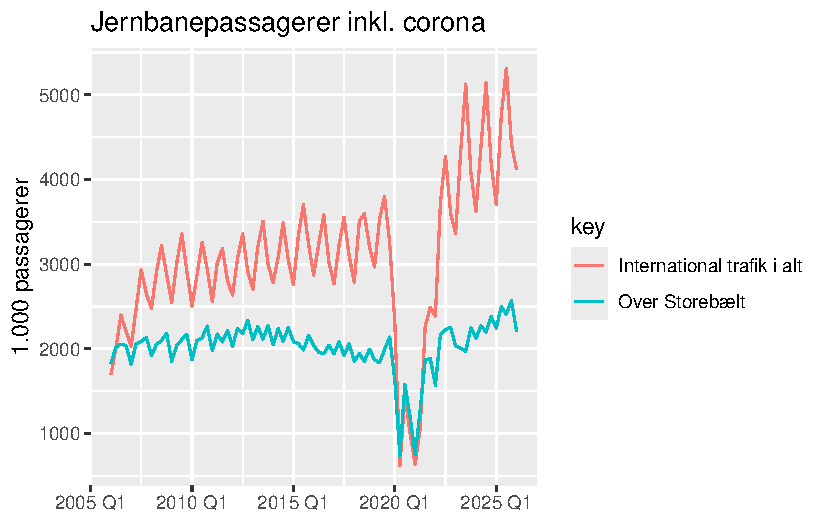
\includegraphics[keepaspectratio]{forecast_files/figure-pdf/fig-autoplot-inkl-1.pdf}}

}

\caption{\label{fig-autoplot-inkl}Jernbanepassagerer}

\end{figure}%

\begin{Shaded}
\begin{Highlighting}[]
\NormalTok{kør}\FunctionTok{\_begge}\NormalTok{(}\ControlFlowTok{function}\NormalTok{(data, titel) \{}
\NormalTok{  data }\SpecialCharTok{\%\textgreater{}\%}
    \FunctionTok{autoplot}\NormalTok{(}\FunctionTok{log}\NormalTok{(x1000\_passagerer)) }\SpecialCharTok{+}
    \FunctionTok{labs}\NormalTok{(}\AttributeTok{title =}\NormalTok{ titel,}
         \AttributeTok{y     =} \StringTok{"log(1.000 passagerer)"}\NormalTok{,}
         \AttributeTok{x     =} \ConstantTok{NULL}\NormalTok{)}
\NormalTok{\})}
\end{Highlighting}
\end{Shaded}

\begin{figure}[H]

\centering{

\pandocbounded{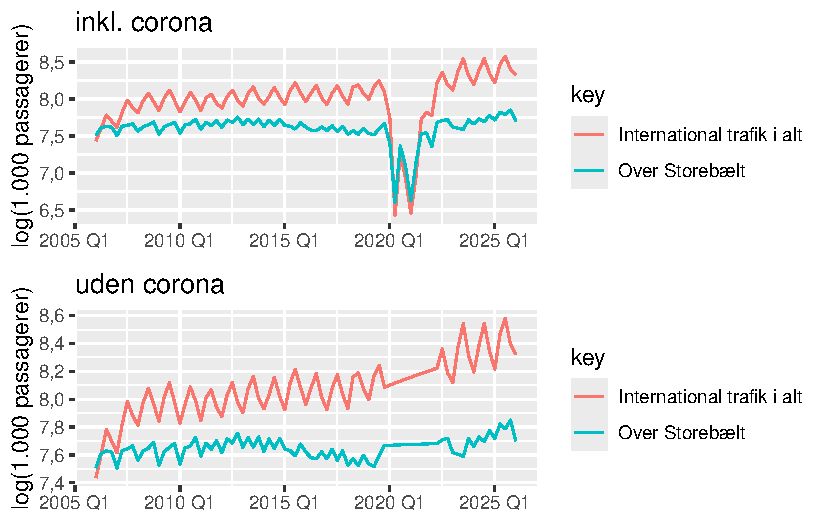
\includegraphics[keepaspectratio]{forecast_files/figure-pdf/fig-log-inkl-1.pdf}}

}

\caption{\label{fig-log-inkl}Log-transformerede jernbanepassagerer}

\end{figure}%

Begge serier viser en opadgående trend fra 2006 til 2019 med et markant
dyk under coronaperioden i 2020. Log-transformationen stabiliserer
variansen og gør sæsonudslagene mere konstante over tid.

\newpage

\subsection{Sæsonplot}\label{suxe6sonplot}

\begin{Shaded}
\begin{Highlighting}[]
\NormalTok{kør}\FunctionTok{\_begge}\NormalTok{(}\ControlFlowTok{function}\NormalTok{(data, titel) \{}
\NormalTok{  data }\SpecialCharTok{\%\textgreater{}\%}
    \FunctionTok{gg\_season}\NormalTok{(x1000\_passagerer) }\SpecialCharTok{+}
    \FunctionTok{labs}\NormalTok{(}\AttributeTok{title =}\NormalTok{ titel,}
         \AttributeTok{y     =} \StringTok{"1.000 passagerer"}\NormalTok{,}
         \AttributeTok{x     =} \ConstantTok{NULL}\NormalTok{)}
\NormalTok{\})}
\end{Highlighting}
\end{Shaded}

\begin{figure}[H]

\centering{

\pandocbounded{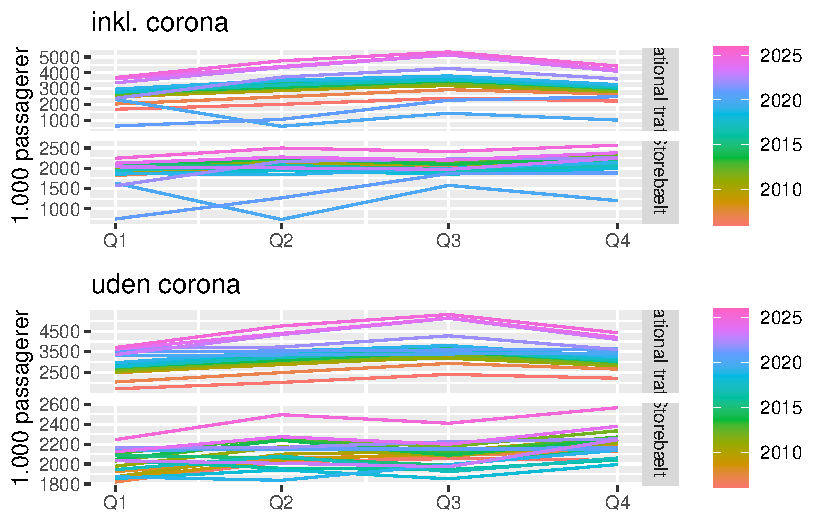
\includegraphics[keepaspectratio]{forecast_files/figure-pdf/fig-saeson-inkl-1.pdf}}

}

\caption{\label{fig-saeson-inkl}Sæsonplot}

\end{figure}%

Sæsonplottene bekræfter et konsistent Q3 peak på tværs af alle år for
international trafik. For Over Storebælt er sæsonudslaget mindre
synligt, da forskellen mellem Q1 \& Q3 er mindre end for international
trafik. I det interpolerede datasæt fremstår alle år med næsten
parallelle forløb, hvilket vidner om et homogent sæsonmønster uden
strukturbrud.

\begin{Shaded}
\begin{Highlighting}[]
\NormalTok{kør}\FunctionTok{\_begge}\NormalTok{(}\ControlFlowTok{function}\NormalTok{(data, titel) \{}
\NormalTok{  data }\SpecialCharTok{\%\textgreater{}\%}
    \FunctionTok{gg\_subseries}\NormalTok{(x1000\_passagerer) }\SpecialCharTok{+}
    \FunctionTok{labs}\NormalTok{(}\AttributeTok{title =}\NormalTok{ titel,}
         \AttributeTok{y     =} \StringTok{"1.000 passagerer"}\NormalTok{,}
         \AttributeTok{x     =} \ConstantTok{NULL}\NormalTok{)}
\NormalTok{\})}
\end{Highlighting}
\end{Shaded}

\begin{figure}[H]

\centering{

\pandocbounded{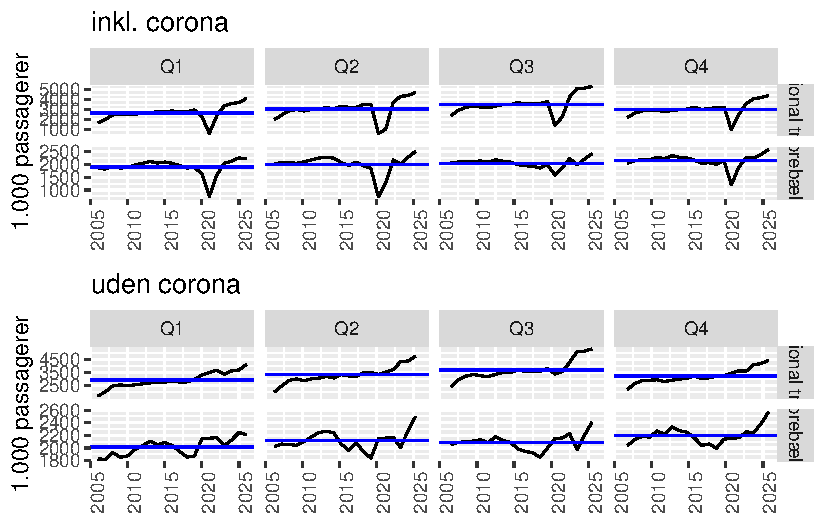
\includegraphics[keepaspectratio]{forecast_files/figure-pdf/fig-subserie-inkl-1.pdf}}

}

\caption{\label{fig-subserie-inkl}Subserie-plot}

\end{figure}%

Begge serier viser et tydeligt sæsonmønster med toppe i tredje kvartal
(Q3) og bund i første kvartal (Q1), samt opadgående trend fra 2006 til
2026 med undtagelse af coronaperioden (2020-2021).

\newpage

\subsection{ACF og PACF}\label{acf-og-pacf}

\begin{Shaded}
\begin{Highlighting}[]
\NormalTok{jernbanedata }\SpecialCharTok{\%\textgreater{}\%}
  \FunctionTok{filter}\NormalTok{(key }\SpecialCharTok{==} \StringTok{"International trafik i alt"}\NormalTok{) }\SpecialCharTok{\%\textgreater{}\%}
  \FunctionTok{mutate}\NormalTok{(}\AttributeTok{x1000\_passagerer =} \FunctionTok{log}\NormalTok{(x1000\_passagerer)) }\SpecialCharTok{\%\textgreater{}\%}
  \FunctionTok{gg\_tsdisplay}\NormalTok{(x1000\_passagerer, }\AttributeTok{plot\_type =} \StringTok{"partial"}\NormalTok{, }\AttributeTok{lag\_max =} \DecValTok{24}\NormalTok{) }\SpecialCharTok{+}
  \FunctionTok{labs}\NormalTok{(}\AttributeTok{title =} \StringTok{"ACF + PACF (log, inkl. corona)"}\NormalTok{)}
\end{Highlighting}
\end{Shaded}

\begin{figure}[H]

\centering{

\pandocbounded{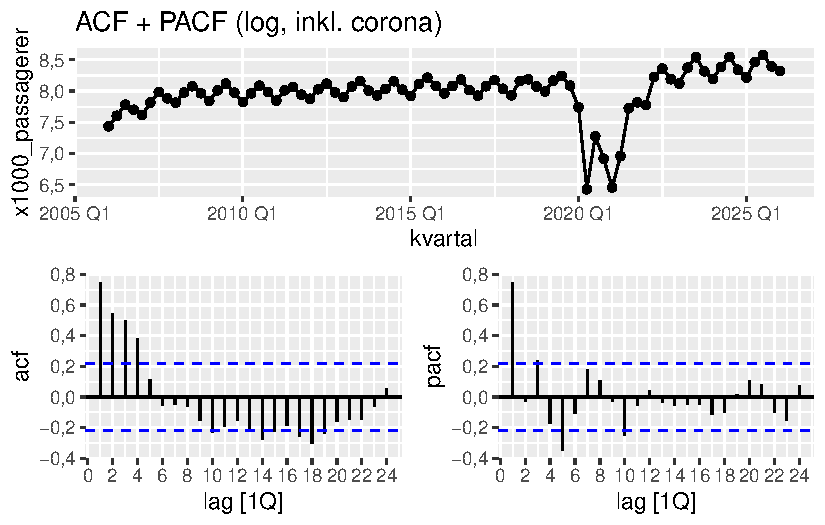
\includegraphics[keepaspectratio]{forecast_files/figure-pdf/fig-acf-int-inkl-1.pdf}}

}

\caption{\label{fig-acf-int-inkl}ACF + PACF -- International trafik i
alt (log, inkl. corona)}

\end{figure}%

\begin{Shaded}
\begin{Highlighting}[]
\NormalTok{jernbanedata }\SpecialCharTok{\%\textgreater{}\%}
  \FunctionTok{filter}\NormalTok{(key }\SpecialCharTok{==} \StringTok{"Over Storebælt"}\NormalTok{) }\SpecialCharTok{\%\textgreater{}\%}
  \FunctionTok{mutate}\NormalTok{(}\AttributeTok{x1000\_passagerer =} \FunctionTok{log}\NormalTok{(x1000\_passagerer)) }\SpecialCharTok{\%\textgreater{}\%}
  \FunctionTok{gg\_tsdisplay}\NormalTok{(x1000\_passagerer, }\AttributeTok{plot\_type =} \StringTok{"partial"}\NormalTok{, }\AttributeTok{lag\_max =} \DecValTok{24}\NormalTok{) }\SpecialCharTok{+}
  \FunctionTok{labs}\NormalTok{(}\AttributeTok{title =} \StringTok{"ACF + PACF (log, inkl. corona)"}\NormalTok{)}
\end{Highlighting}
\end{Shaded}

\begin{figure}[H]

\centering{

\pandocbounded{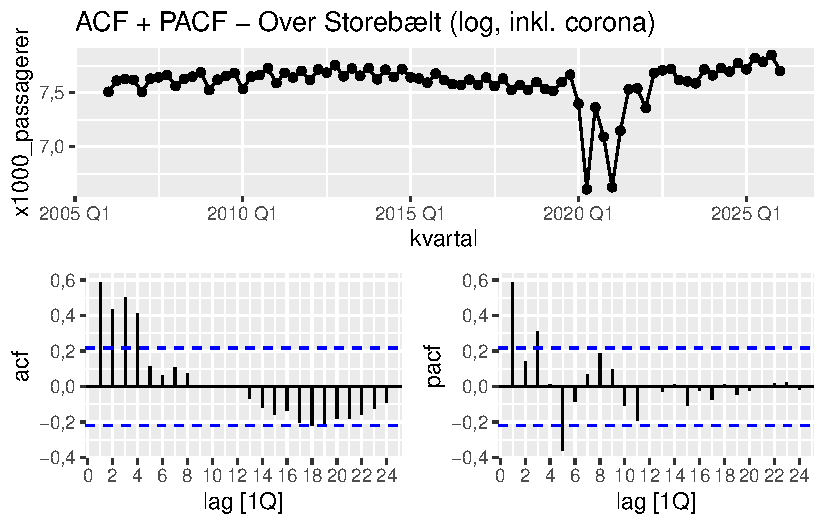
\includegraphics[keepaspectratio]{forecast_files/figure-pdf/fig-acf-osb-inkl-1.pdf}}

}

\caption{\label{fig-acf-osb-inkl}ACF + PACF -- Over Storebælt (log,
inkl. corona)}

\end{figure}%

\begin{Shaded}
\begin{Highlighting}[]
\NormalTok{jernbanedata\_corona }\SpecialCharTok{\%\textgreater{}\%}
  \FunctionTok{filter}\NormalTok{(key }\SpecialCharTok{==} \StringTok{"International trafik i alt"}\NormalTok{) }\SpecialCharTok{\%\textgreater{}\%}
  \FunctionTok{mutate}\NormalTok{(}\AttributeTok{x1000\_passagerer =} \FunctionTok{log}\NormalTok{(x1000\_passagerer)) }\SpecialCharTok{\%\textgreater{}\%}
  \FunctionTok{gg\_tsdisplay}\NormalTok{(x1000\_passagerer, }\AttributeTok{plot\_type =} \StringTok{"partial"}\NormalTok{, }\AttributeTok{lag\_max =} \DecValTok{24}\NormalTok{) }\SpecialCharTok{+}
  \FunctionTok{labs}\NormalTok{(}\AttributeTok{title =} \StringTok{"ACF + PACF (log, uden corona)"}\NormalTok{)}
\end{Highlighting}
\end{Shaded}

\begin{figure}[H]

\centering{

\pandocbounded{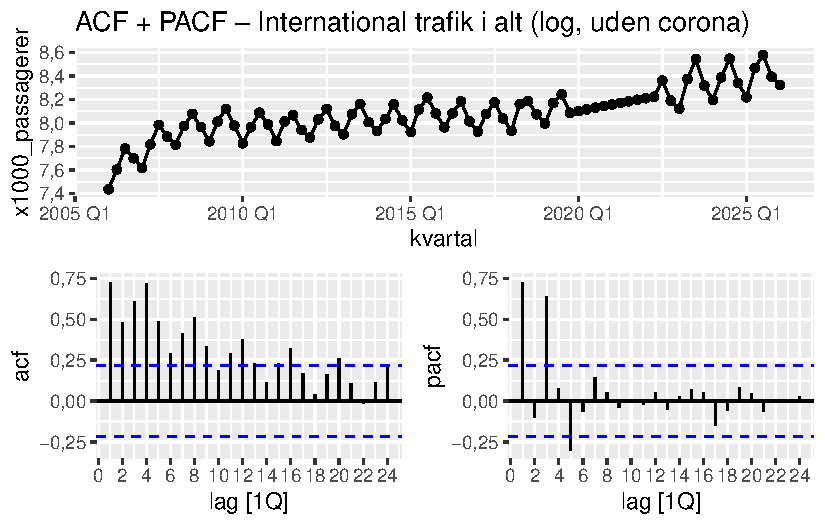
\includegraphics[keepaspectratio]{forecast_files/figure-pdf/fig-acf-int-uden-1.pdf}}

}

\caption{\label{fig-acf-int-uden}ACF + PACF -- International trafik i
alt (log, uden corona)}

\end{figure}%

\begin{Shaded}
\begin{Highlighting}[]
\NormalTok{jernbanedata\_corona }\SpecialCharTok{\%\textgreater{}\%}
  \FunctionTok{filter}\NormalTok{(key }\SpecialCharTok{==} \StringTok{"Over Storebælt"}\NormalTok{) }\SpecialCharTok{\%\textgreater{}\%}
  \FunctionTok{mutate}\NormalTok{(}\AttributeTok{x1000\_passagerer =} \FunctionTok{log}\NormalTok{(x1000\_passagerer)) }\SpecialCharTok{\%\textgreater{}\%}
  \FunctionTok{gg\_tsdisplay}\NormalTok{(x1000\_passagerer, }\AttributeTok{plot\_type =} \StringTok{"partial"}\NormalTok{, }\AttributeTok{lag\_max =} \DecValTok{24}\NormalTok{) }\SpecialCharTok{+}
  \FunctionTok{labs}\NormalTok{(}\AttributeTok{title =} \StringTok{"ACF + PACF (log, uden corona)"}\NormalTok{)}
\end{Highlighting}
\end{Shaded}

\begin{figure}[H]

\centering{

\pandocbounded{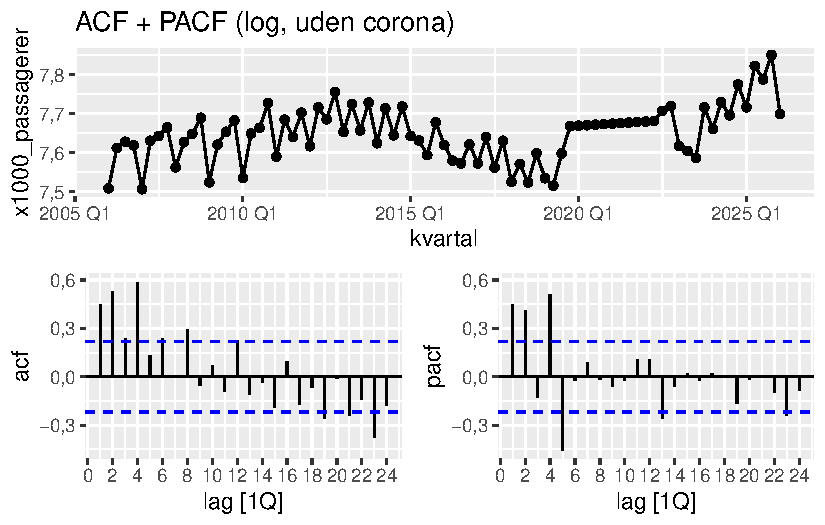
\includegraphics[keepaspectratio]{forecast_files/figure-pdf/fig-acf-osb-uden-1.pdf}}

}

\caption{\label{fig-acf-osb-uden}ACF + PACF -- Over Storebælt (log, uden
corona)}

\end{figure}%

ACF Plottene for rådata (Log skala) viser lag som, eksponentiel aftagen
uden klart cutoff, som er normalt for ikke stationære serier med trend.
Signifikante toppe optræder ved lag 4 \& 8. (kvartalsvis sæsonperiode)

PACF-plottene afskæres efter lag 1--2 for den ordinære komponent,
hvilket indikerer en AR-struktur. For den sæsonale komponent er PACF
signifikant ved lag 4 for international trafik, hvilket peger på en
sæsonel AR-komponent.

Samlet begrunder dette kandidatmodeller med ARIMA(p,d,q)(P,D,Q){[}4{]},
hvor de konkrete ordener bestemmes via stationaritetstest og
AICc-sammenligning.

\newpage

\begin{Shaded}
\begin{Highlighting}[]
\NormalTok{jernbanedata }\SpecialCharTok{\%\textgreater{}\%}
  \FunctionTok{filter}\NormalTok{(key }\SpecialCharTok{==} \StringTok{"Over Storebælt"}\NormalTok{) }\SpecialCharTok{\%\textgreater{}\%}
  \FunctionTok{gg\_lag}\NormalTok{(x1000\_passagerer, }\AttributeTok{geom =} \StringTok{"point"}\NormalTok{) }\SpecialCharTok{+}
  \FunctionTok{labs}\NormalTok{(}\AttributeTok{x =} \StringTok{"lag(x1000\_passagerer, k)"}\NormalTok{)}
\end{Highlighting}
\end{Shaded}

\begin{figure}[H]

\centering{

\pandocbounded{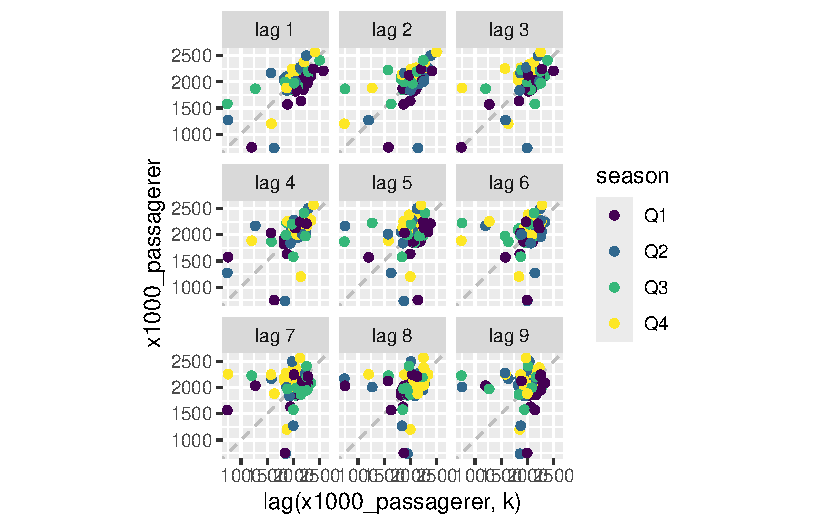
\includegraphics[keepaspectratio]{forecast_files/figure-pdf/fig-lag-osb-inkl-1.pdf}}

}

\caption{\label{fig-lag-osb-inkl}Lag-plot -- Over Storebælt (inkl.
corona)}

\end{figure}%

\begin{Shaded}
\begin{Highlighting}[]
\NormalTok{jernbanedata }\SpecialCharTok{\%\textgreater{}\%}
  \FunctionTok{filter}\NormalTok{(key }\SpecialCharTok{==} \StringTok{"International trafik i alt"}\NormalTok{) }\SpecialCharTok{\%\textgreater{}\%}
  \FunctionTok{gg\_lag}\NormalTok{(x1000\_passagerer, }\AttributeTok{geom =} \StringTok{"point"}\NormalTok{) }\SpecialCharTok{+}
  \FunctionTok{labs}\NormalTok{(}\AttributeTok{x =} \StringTok{"lag(x1000\_passagerer, k)"}\NormalTok{)}
\end{Highlighting}
\end{Shaded}

\begin{figure}[H]

\centering{

\pandocbounded{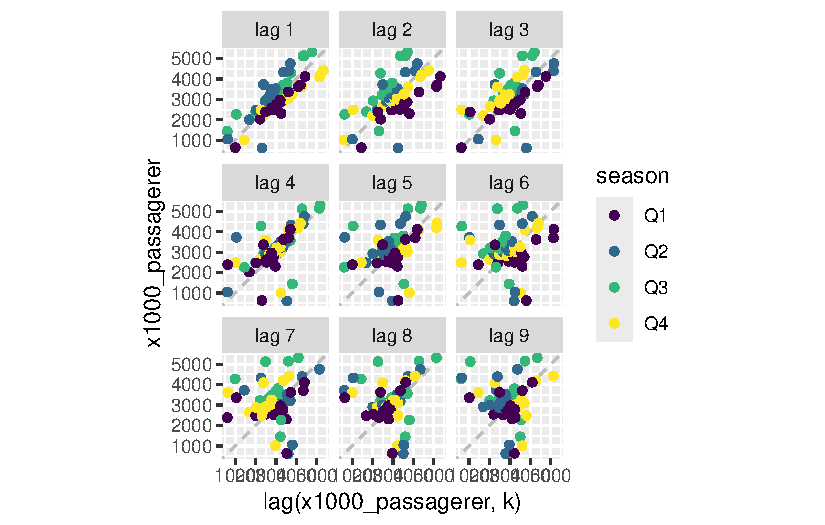
\includegraphics[keepaspectratio]{forecast_files/figure-pdf/fig-lag-int-inkl-1.pdf}}

}

\caption{\label{fig-lag-int-inkl}Lag-plot -- International trafik i alt
(inkl. corona)}

\end{figure}%

\begin{Shaded}
\begin{Highlighting}[]
\NormalTok{jernbanedata\_corona }\SpecialCharTok{\%\textgreater{}\%}
  \FunctionTok{filter}\NormalTok{(key }\SpecialCharTok{==} \StringTok{"Over Storebælt"}\NormalTok{) }\SpecialCharTok{\%\textgreater{}\%}
  \FunctionTok{gg\_lag}\NormalTok{(x1000\_passagerer, }\AttributeTok{geom =} \StringTok{"point"}\NormalTok{) }\SpecialCharTok{+}
  \FunctionTok{labs}\NormalTok{(}\AttributeTok{x =} \StringTok{"lag(x1000\_passagerer, k)"}\NormalTok{)}
\end{Highlighting}
\end{Shaded}

\begin{figure}[H]

\centering{

\pandocbounded{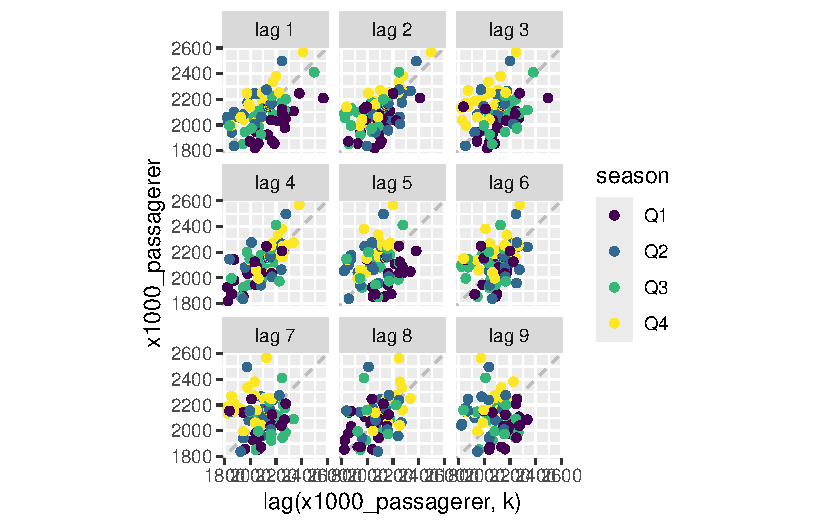
\includegraphics[keepaspectratio]{forecast_files/figure-pdf/fig-lag-osb-uden-1.pdf}}

}

\caption{\label{fig-lag-osb-uden}Lag-plot -- Over Storebælt (uden
corona)}

\end{figure}%

\begin{Shaded}
\begin{Highlighting}[]
\NormalTok{jernbanedata\_corona }\SpecialCharTok{\%\textgreater{}\%}
  \FunctionTok{filter}\NormalTok{(key }\SpecialCharTok{==} \StringTok{"International trafik i alt"}\NormalTok{) }\SpecialCharTok{\%\textgreater{}\%}
  \FunctionTok{gg\_lag}\NormalTok{(x1000\_passagerer, }\AttributeTok{geom =} \StringTok{"point"}\NormalTok{) }\SpecialCharTok{+}
  \FunctionTok{labs}\NormalTok{(}\AttributeTok{x =} \StringTok{"lag(x1000\_passagerer, k)"}\NormalTok{)}
\end{Highlighting}
\end{Shaded}

\begin{figure}[H]

\centering{

\pandocbounded{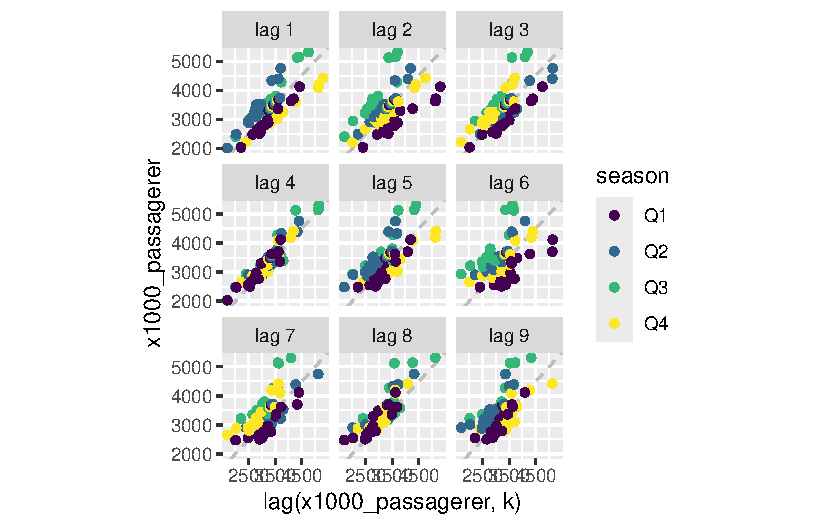
\includegraphics[keepaspectratio]{forecast_files/figure-pdf/fig-lag-int-uden-1.pdf}}

}

\caption{\label{fig-lag-int-uden}Lag-plot -- International trafik i alt
(uden corona)}

\end{figure}%

Lag-plottene viser sammenhængen mellem en observation og dens tidligere
værdier. En tydelig lineær sammenhæng ved lag 4 bekræfter det
kvartalsvise sæsonmønster i begge serier.

\newpage

\subsection{Deskriptive statistikker}\label{deskriptive-statistikker}

\begin{table}

\caption{\label{tbl-desk-inkl}Deskriptive statistikker}

\centering{

\begin{Shaded}
\begin{Highlighting}[]
\NormalTok{kør}\FunctionTok{\_begge\_tbl}\NormalTok{(}\ControlFlowTok{function}\NormalTok{(data, titel) \{}
\NormalTok{  data }\SpecialCharTok{\%\textgreater{}\%}
    \FunctionTok{as\_tibble}\NormalTok{() }\SpecialCharTok{\%\textgreater{}\%}
    \FunctionTok{group\_by}\NormalTok{(key) }\SpecialCharTok{\%\textgreater{}\%}
    \FunctionTok{summarise}\NormalTok{(}
      \AttributeTok{N      =} \FunctionTok{sum}\NormalTok{(}\SpecialCharTok{!}\FunctionTok{is.na}\NormalTok{(x1000\_passagerer)),}
      \AttributeTok{mean   =} \FunctionTok{mean}\NormalTok{(x1000\_passagerer,          }\AttributeTok{na.rm =} \ConstantTok{TRUE}\NormalTok{),}
      \AttributeTok{median =} \FunctionTok{median}\NormalTok{(x1000\_passagerer,         }\AttributeTok{na.rm =} \ConstantTok{TRUE}\NormalTok{),}
      \AttributeTok{sd     =} \FunctionTok{sd}\NormalTok{(x1000\_passagerer,             }\AttributeTok{na.rm =} \ConstantTok{TRUE}\NormalTok{),}
      \AttributeTok{Q1     =} \FunctionTok{quantile}\NormalTok{(x1000\_passagerer, }\FloatTok{0.25}\NormalTok{, }\AttributeTok{na.rm =} \ConstantTok{TRUE}\NormalTok{),}
      \AttributeTok{Q3     =} \FunctionTok{quantile}\NormalTok{(x1000\_passagerer, }\FloatTok{0.75}\NormalTok{, }\AttributeTok{na.rm =} \ConstantTok{TRUE}\NormalTok{),}
      \AttributeTok{min    =} \FunctionTok{min}\NormalTok{(x1000\_passagerer,            }\AttributeTok{na.rm =} \ConstantTok{TRUE}\NormalTok{),}
      \AttributeTok{max    =} \FunctionTok{max}\NormalTok{(x1000\_passagerer,            }\AttributeTok{na.rm =} \ConstantTok{TRUE}\NormalTok{)}
\NormalTok{    ) }\SpecialCharTok{\%\textgreater{}\%}
   \FunctionTok{kbl}\NormalTok{(}\AttributeTok{digits =} \DecValTok{1}\NormalTok{, }\AttributeTok{booktabs =} \ConstantTok{TRUE}\NormalTok{) }\SpecialCharTok{\%\textgreater{}\%}
  \FunctionTok{kable\_styling}\NormalTok{(}\AttributeTok{latex\_options =} \FunctionTok{c}\NormalTok{(}\StringTok{"striped"}\NormalTok{, }\StringTok{"hold\_position"}\NormalTok{))}
  
\NormalTok{\})}
\end{Highlighting}
\end{Shaded}

\centering
\begin{tabular}[t]{lrrrrrrrr}
\toprule
key & N & mean & median & sd & Q1 & Q3 & min & max\\
\midrule
\cellcolor{gray!10}{International trafik i alt} & \cellcolor{gray!10}{81} & \cellcolor{gray!10}{3075,8} & \cellcolor{gray!10}{3049} & \cellcolor{gray!10}{892,9} & \cellcolor{gray!10}{2654} & \cellcolor{gray!10}{3528} & \cellcolor{gray!10}{619} & \cellcolor{gray!10}{5315}\\
Over Storebælt & 81 & 2019,4 & 2061 & 300,7 & 1945 & 2177 & 738 & 2568\\
\bottomrule
\end{tabular}

\centering
\begin{tabular}[t]{lrrrrrrrr}
\toprule
key & N & mean & median & sd & Q1 & Q3 & min & max\\
\midrule
\cellcolor{gray!10}{International trafik i alt} & \cellcolor{gray!10}{81} & \cellcolor{gray!10}{3287,9} & \cellcolor{gray!10}{3237} & \cellcolor{gray!10}{677,9} & \cellcolor{gray!10}{2879} & \cellcolor{gray!10}{3584,2} & \cellcolor{gray!10}{1696} & \cellcolor{gray!10}{5315}\\
Over Storebælt & 81 & 2104,4 & 2108 & 147,7 & 2023 & 2177,0 & 1820 & 2568\\
\bottomrule
\end{tabular}

}

\end{table}%

International trafik i alt viser et gennemsnit på 3076 passagerer og en
varianskoeffecient på 29\% (SD=893), med et spænd fra 619 til 5.315
drevet af coronanedgangen. Over storebælt er trafikken væsentlig mere
stabil: Gennemsnit 2.019 og varianskoeffecient på 15\% (SD=301).

Den markant større spredning i International Trafik begrunder anvendelse
af en varians stabiliserende transformation, samt opdeling i 2 seperate
datasæt.

\newpage

\subsection{STL-features: trend- og
sæsonstyrke}\label{stl-features-trend--og-suxe6sonstyrke}

\begin{table}

\caption{\label{tbl-stl-inkl}Trend- og sæsonstyrke inkl. corona}

\centering{

\begin{Shaded}
\begin{Highlighting}[]
\NormalTok{kør}\FunctionTok{\_begge\_tbl}\NormalTok{(}\ControlFlowTok{function}\NormalTok{(data, titel) \{}
\NormalTok{  data }\SpecialCharTok{\%\textgreater{}\%}
    \FunctionTok{features}\NormalTok{(x1000\_passagerer, feat\_stl) }\SpecialCharTok{\%\textgreater{}\%}
    \FunctionTok{select}\NormalTok{(trend\_strength, seasonal\_strength\_year) }\SpecialCharTok{\%\textgreater{}\%}
    \FunctionTok{kbl}\NormalTok{(}\AttributeTok{digits   =} \DecValTok{3}\NormalTok{, }\AttributeTok{booktabs =} \ConstantTok{TRUE}\NormalTok{) }\SpecialCharTok{\%\textgreater{}\%}
    \FunctionTok{kable\_styling}\NormalTok{(}\AttributeTok{latex\_options =} \FunctionTok{c}\NormalTok{(}\StringTok{"striped"}\NormalTok{, }\StringTok{"hold\_position"}\NormalTok{))}
\NormalTok{\})}
\end{Highlighting}
\end{Shaded}

\centering
\begin{tabular}[t]{rr}
\toprule
trend\_strength & seasonal\_strength\_year\\
\midrule
\cellcolor{gray!10}{0,965} & \cellcolor{gray!10}{0,813}\\
0,866 & 0,513\\
\bottomrule
\end{tabular}

\centering
\begin{tabular}[t]{rr}
\toprule
trend\_strength & seasonal\_strength\_year\\
\midrule
\cellcolor{gray!10}{0,962} & \cellcolor{gray!10}{0,856}\\
0,908 & 0,800\\
\bottomrule
\end{tabular}

}

\end{table}%

STL features bekræfter de visuelle observationer kvantitativt.
International trafik i alt har høj trend styrke (0,965 \& 0,962
inkl/ekskl. corona) og sæsonstyrke (0,813/0,856) hvor coronaperioden kun
dæmper sæsonmønstret minimalt. Over storebælt er effekten mere markant,
trend styrken stiger fra 0,866 til 0,908 og sæsonstyrken øges fra 0,513
til 0,800 uden corona. Dette betyder at pandemiens ekstreme udsving
indikerer at sæsonkomponenter er nødvendige i både ETS \& SARIMA.

\newpage

\section{Transformation}\label{transformation}

\subsection{Box-Cox og Guerrero}\label{box-cox-og-guerrero}

\begin{table}

\caption{\label{tbl-guerrero-inkl}Guerrero-optimeret Box-Cox lambda
inkl. corona}

\centering{

\begin{Shaded}
\begin{Highlighting}[]
\NormalTok{kør}\FunctionTok{\_begge\_tbl}\NormalTok{(}\ControlFlowTok{function}\NormalTok{(data, titel) \{}
\NormalTok{  data }\SpecialCharTok{\%\textgreater{}\%}
    \FunctionTok{features}\NormalTok{(x1000\_passagerer, }\AttributeTok{features =}\NormalTok{ guerrero) }\SpecialCharTok{\%\textgreater{}\%}
    \FunctionTok{rename}\NormalTok{(}\AttributeTok{Lambda\_Guerrero =}\NormalTok{ lambda\_guerrero) }\SpecialCharTok{\%\textgreater{}\%}
    \FunctionTok{kbl}\NormalTok{(}\AttributeTok{digits   =} \DecValTok{3}\NormalTok{, }\AttributeTok{booktabs =} \ConstantTok{TRUE}\NormalTok{) }\SpecialCharTok{\%\textgreater{}\%}
    \FunctionTok{kable\_styling}\NormalTok{(}\AttributeTok{latex\_options =} \FunctionTok{c}\NormalTok{(}\StringTok{"striped"}\NormalTok{, }\StringTok{"hold\_position"}\NormalTok{))}
\NormalTok{\})}
\end{Highlighting}
\end{Shaded}

\centering
\begin{tabular}[t]{lr}
\toprule
key & Lambda\_Guerrero\\
\midrule
\cellcolor{gray!10}{International trafik i alt} & \cellcolor{gray!10}{0,855}\\
Over Storebælt & 2,000\\
\bottomrule
\end{tabular}

\centering
\begin{tabular}[t]{lr}
\toprule
key & Lambda\_Guerrero\\
\midrule
\cellcolor{gray!10}{International trafik i alt} & \cellcolor{gray!10}{-0,606}\\
Over Storebælt & -0,051\\
\bottomrule
\end{tabular}

}

\end{table}%

Guerrero metoden estimerer inkl. corona en lambda på 0,855
(international) og Lambda 2,00 (storebælt). Disse værdier er dog
kunstigt oppustede af coronaperiodens udsving, og er ikke repræsentative
for den underliggende varians struktur. Det corona rensede datasæt giver
et mere retvisende billede med lambda -0,606 (international) og -0,051
(Storebælt), hvor storebælt er tæt på 0, og dermed understøtter log
transformation. Log transformationen fastholdes konsekvent for begge
serier i al efterfølgende modellering og fable tilbagekalkulerer
automatisk til originalskala ved forecast. Dette understøttes af figur 1
\& 2

\section{Stationaritet og
differentiering}\label{stationaritet-og-differentiering}

KPSS testen kan ikke afvise stationaritets hypotesen (P \textgreater{}
0,10) for nogen serie på log skala. trods synlig opadgående trend,
afvises den ikke som ikke stationær Dette skyldes coronaperiodens dyk og
efterfølgende genopretning der skaber et mean reversionsmønster.
Konsistent returnerer nsdiffs og ndiffs begge 0, inkl. corona, og
Auto-ARIMA vælger ARIMA(1,0,0)(1,0,0){[}4{]} og
ARIMA(1,0,0)(0,0,1){[}4{]} uden differentiering. På det corona-rensede
datasæt, hvor trendstrukturen er renere, vælger Auto-ARIMA D = 1 for
begge serier.

Testresultaterne fremgår af \textbf{?@sec-bilag-a}.

\newpage

\begin{Shaded}
\begin{Highlighting}[]
\NormalTok{jernbanedata }\SpecialCharTok{\%\textgreater{}\%}
  \FunctionTok{filter}\NormalTok{(key }\SpecialCharTok{==} \StringTok{"International trafik i alt"}\NormalTok{) }\SpecialCharTok{\%\textgreater{}\%}
  \FunctionTok{as\_tibble}\NormalTok{() }\SpecialCharTok{\%\textgreater{}\%}
  \FunctionTok{transmute}\NormalTok{(}
\NormalTok{    kvartal,}
    \StringTok{\textasciigrave{}}\AttributeTok{log(passagerer)}\StringTok{\textasciigrave{}}     \OtherTok{=} \FunctionTok{log}\NormalTok{(x1000\_passagerer),}
    \StringTok{\textasciigrave{}}\AttributeTok{Δlog (d=1)}\StringTok{\textasciigrave{}}           \OtherTok{=} \FunctionTok{difference}\NormalTok{(}\FunctionTok{log}\NormalTok{(x1000\_passagerer), }\DecValTok{1}\NormalTok{),}
    \StringTok{\textasciigrave{}}\AttributeTok{Δ₄log (D=1, lag=4)}\StringTok{\textasciigrave{}}  \OtherTok{=} \FunctionTok{difference}\NormalTok{(}\FunctionTok{log}\NormalTok{(x1000\_passagerer), }\DecValTok{4}\NormalTok{),}
    \StringTok{\textasciigrave{}}\AttributeTok{ΔΔ₄log (d=1, D=1)}\StringTok{\textasciigrave{}}   \OtherTok{=} \FunctionTok{difference}\NormalTok{(}\FunctionTok{difference}\NormalTok{(}\FunctionTok{log}\NormalTok{(x1000\_passagerer), }\DecValTok{4}\NormalTok{), }\DecValTok{1}\NormalTok{)}
\NormalTok{  ) }\SpecialCharTok{\%\textgreater{}\%}
  \FunctionTok{pivot\_longer}\NormalTok{(}\SpecialCharTok{{-}}\NormalTok{kvartal, }\AttributeTok{names\_to =} \StringTok{"Type"}\NormalTok{, }\AttributeTok{values\_to =} \StringTok{"Værdi"}\NormalTok{) }\SpecialCharTok{\%\textgreater{}\%}
  \FunctionTok{mutate}\NormalTok{(}\AttributeTok{Type =} \FunctionTok{factor}\NormalTok{(Type, }\AttributeTok{levels =} \FunctionTok{c}\NormalTok{(}
    \StringTok{"log(passagerer)"}\NormalTok{, }\StringTok{"Δlog (d=1)"}\NormalTok{, }\StringTok{"Δ₄log (D=1, lag=4)"}\NormalTok{, }\StringTok{"ΔΔ₄log (d=1, D=1)"}
\NormalTok{  ))) }\SpecialCharTok{\%\textgreater{}\%}
  \FunctionTok{ggplot}\NormalTok{(}\FunctionTok{aes}\NormalTok{(}\AttributeTok{x =}\NormalTok{ kvartal, }\AttributeTok{y =}\NormalTok{ Værdi)) }\SpecialCharTok{+}
  \FunctionTok{geom\_line}\NormalTok{() }\SpecialCharTok{+}
  \FunctionTok{facet\_grid}\NormalTok{(}\FunctionTok{vars}\NormalTok{(Type), }\AttributeTok{scales =} \StringTok{"free\_y"}\NormalTok{) }\SpecialCharTok{+}
  \FunctionTok{labs}\NormalTok{(}\AttributeTok{title =} \StringTok{"Differentieringstrin – International trafik i alt"}\NormalTok{,}
       \AttributeTok{y =} \ConstantTok{NULL}\NormalTok{, }\AttributeTok{x =} \ConstantTok{NULL}\NormalTok{)}
\end{Highlighting}
\end{Shaded}

\begin{figure}[H]

\centering{

\pandocbounded{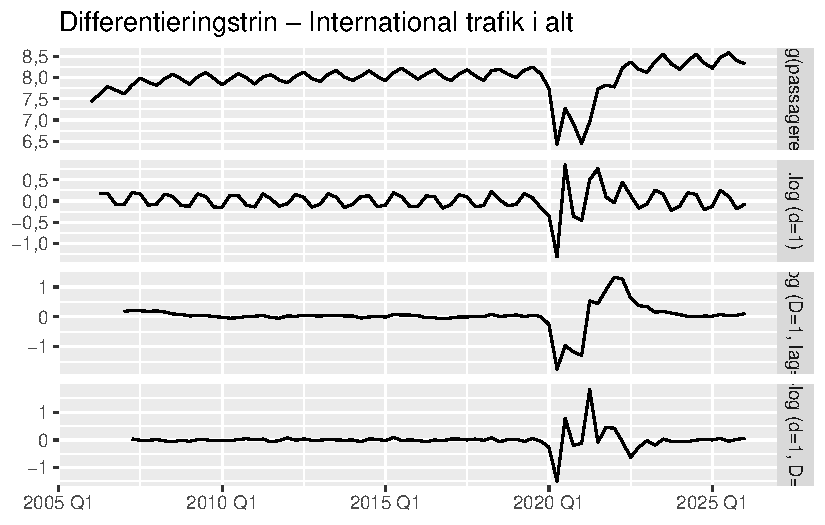
\includegraphics[keepaspectratio]{forecast_files/figure-pdf/fig-diff-trin-int-1.pdf}}

}

\caption{\label{fig-diff-trin-int}Differentieringstrin -- International
trafik i alt}

\end{figure}%

Figuren viser fire differentieringstrin for International trafik i alt.
Sæsondifferentiering (D=1, lag=4) fjerner det periodiske mønster og
giver en tilnærmelsesvis stationær serie, hvilket bekræfter at kun D=1
er nødvendigt.

\newpage

\begin{Shaded}
\begin{Highlighting}[]
\NormalTok{jernbanedata }\SpecialCharTok{\%\textgreater{}\%}
  \FunctionTok{filter}\NormalTok{(key }\SpecialCharTok{==} \StringTok{"International trafik i alt"}\NormalTok{) }\SpecialCharTok{\%\textgreater{}\%}
  \FunctionTok{gg\_tsdisplay}\NormalTok{(}\FunctionTok{difference}\NormalTok{(}\FunctionTok{log}\NormalTok{(x1000\_passagerer), }\AttributeTok{lag =} \DecValTok{4}\NormalTok{),}
               \AttributeTok{plot\_type =} \StringTok{"partial"}\NormalTok{, }\AttributeTok{lag\_max =} \DecValTok{24}\NormalTok{) }\SpecialCharTok{+}
  \FunctionTok{labs}\NormalTok{(}\AttributeTok{title =} \StringTok{"ACF/PACF – sæsondiff (D=1, lag=4) – International"}\NormalTok{)}
\end{Highlighting}
\end{Shaded}

\begin{figure}[H]

\centering{

\pandocbounded{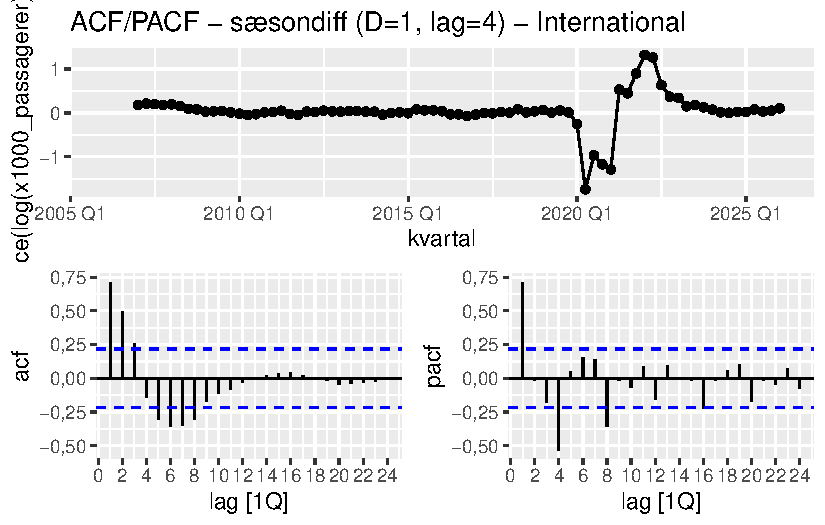
\includegraphics[keepaspectratio]{forecast_files/figure-pdf/fig-acf-sdiff-int-1.pdf}}

}

\caption{\label{fig-acf-sdiff-int}ACF/PACF -- sæsondiff (D=1, lag=4) --
International}

\end{figure}%

ACF viser signifikante spike ved lag 4 og 8. Dette indikerer
tilbageværende sæsonstruktur efter én sæsondifferentiering. PACF
afskæres derimod efter lag 4, hvilket peger på et sæsonelt AR(1)-led og
understøtter en SAR(1)-specifikation.

\begin{Shaded}
\begin{Highlighting}[]
\NormalTok{jernbanedata }\SpecialCharTok{\%\textgreater{}\%}
  \FunctionTok{filter}\NormalTok{(key }\SpecialCharTok{==} \StringTok{"Over Storebælt"}\NormalTok{) }\SpecialCharTok{\%\textgreater{}\%}
  \FunctionTok{gg\_tsdisplay}\NormalTok{(}\FunctionTok{difference}\NormalTok{(}\FunctionTok{log}\NormalTok{(x1000\_passagerer), }\AttributeTok{lag =} \DecValTok{4}\NormalTok{),}
               \AttributeTok{plot\_type =} \StringTok{"partial"}\NormalTok{, }\AttributeTok{lag\_max =} \DecValTok{24}\NormalTok{) }\SpecialCharTok{+}
  \FunctionTok{labs}\NormalTok{(}\AttributeTok{title =} \StringTok{"ACF/PACF – sæsondiff (D=1, lag=4) – Over Storebælt"}\NormalTok{)}
\end{Highlighting}
\end{Shaded}

\begin{figure}[H]

\centering{

\pandocbounded{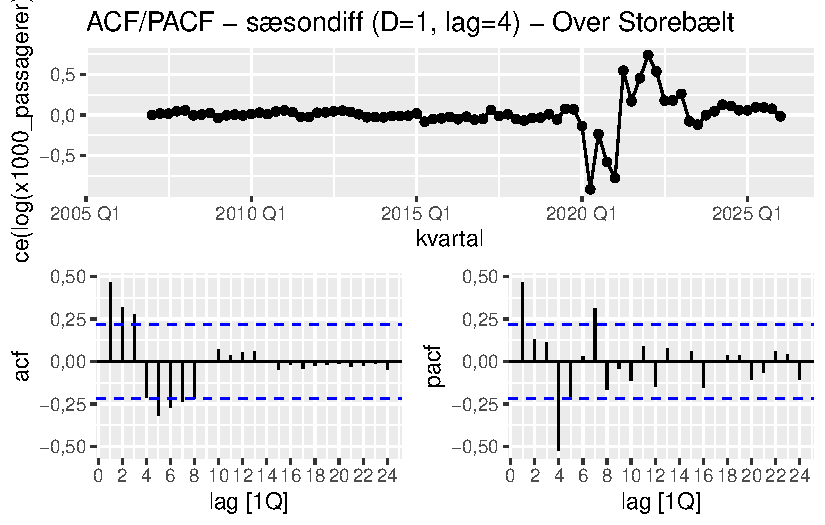
\includegraphics[keepaspectratio]{forecast_files/figure-pdf/fig-acf-sdiff-osb-1.pdf}}

}

\caption{\label{fig-acf-sdiff-osb}ACF/PACF -- sæsondiff (D=1, lag=4) --
Over Storebælt}

\end{figure}%

Dobbelt differentiering udelades, da \texttt{unitroot\_ndiffs}
returnerer d=0 efter D=1. Overdifferentiering forværrer modellen, og
derfor anvendes kun D=1.

\section{STL-dekomposition}\label{stl-dekomposition}

\begin{Shaded}
\begin{Highlighting}[]
\CommentTok{\# STL inkl. corona}
\NormalTok{stl\_comp }\OtherTok{\textless{}{-}} \ControlFlowTok{function}\NormalTok{(data) \{}
\NormalTok{  data }\SpecialCharTok{\%\textgreater{}\%}
    \FunctionTok{model}\NormalTok{(}
      \FunctionTok{STL}\NormalTok{(}\FunctionTok{log}\NormalTok{(x1000\_passagerer) }\SpecialCharTok{\textasciitilde{}} \FunctionTok{trend}\NormalTok{(}\AttributeTok{window =} \DecValTok{7}\NormalTok{) }\SpecialCharTok{+} \FunctionTok{season}\NormalTok{(}\AttributeTok{window =} \StringTok{"periodic"}\NormalTok{),}
          \AttributeTok{robust =} \ConstantTok{TRUE}\NormalTok{)}
\NormalTok{    ) }\SpecialCharTok{\%\textgreater{}\%}
    \FunctionTok{components}\NormalTok{()}
\NormalTok{\}}
\end{Highlighting}
\end{Shaded}

\begin{Shaded}
\begin{Highlighting}[]
\NormalTok{kør}\FunctionTok{\_begge}\NormalTok{(}\ControlFlowTok{function}\NormalTok{(data, titel) \{}
  \FunctionTok{stl\_comp}\NormalTok{(data) }\SpecialCharTok{\%\textgreater{}\%}
    \FunctionTok{as\_tsibble}\NormalTok{() }\SpecialCharTok{\%\textgreater{}\%}
    \FunctionTok{autoplot}\NormalTok{(}\StringTok{\textasciigrave{}}\AttributeTok{log(x1000\_passagerer)}\StringTok{\textasciigrave{}}\NormalTok{, }\AttributeTok{color =} \StringTok{"gray"}\NormalTok{) }\SpecialCharTok{+}
    \FunctionTok{geom\_line}\NormalTok{(}\FunctionTok{aes}\NormalTok{(}\AttributeTok{y =}\NormalTok{ season\_adjust), }\AttributeTok{colour =} \StringTok{"\#0072B2"}\NormalTok{) }\SpecialCharTok{+}
    \FunctionTok{labs}\NormalTok{(}\AttributeTok{title =} \FunctionTok{paste0}\NormalTok{(}\StringTok{"Sæsonjusteret serie – "}\NormalTok{, titel),}
         \AttributeTok{y =} \StringTok{"log(1.000 passagerer)"}\NormalTok{,}
         \AttributeTok{x =} \ConstantTok{NULL}\NormalTok{)}
\NormalTok{\})}
\end{Highlighting}
\end{Shaded}

\begin{figure}[H]

\centering{

\pandocbounded{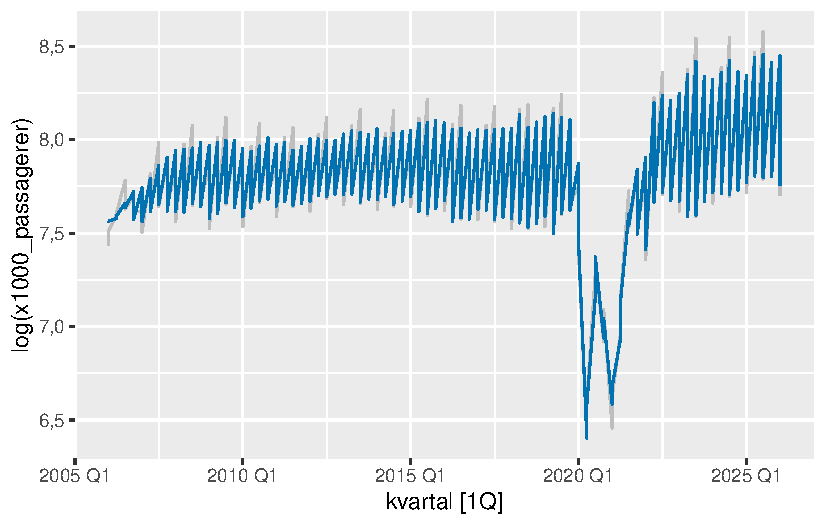
\includegraphics[keepaspectratio]{forecast_files/figure-pdf/fig-stl-adj-inkl-1.pdf}}

}

\caption{\label{fig-stl-adj-inkl}Sæsonjusteret serie -- inkl. corona}

\end{figure}%

Den grå linje viser den rå log-transformerede serie mens den blå linje
viser den sæsonjusterede serie. Den underliggende trend fremstår
tydeligt efter sæsonkomponenten er fjernet.

\begin{Shaded}
\begin{Highlighting}[]
\NormalTok{kør}\FunctionTok{\_begge}\NormalTok{(}\ControlFlowTok{function}\NormalTok{(data, titel) \{}
  \FunctionTok{stl\_comp}\NormalTok{(data) }\SpecialCharTok{\%\textgreater{}\%}
    \FunctionTok{autoplot}\NormalTok{() }\SpecialCharTok{+}
    \FunctionTok{scale\_color\_discrete}\NormalTok{(}\AttributeTok{labels =} \FunctionTok{c}\NormalTok{(}\StringTok{"International trafik i alt"}\NormalTok{, }\StringTok{"Over Storebælt"}\NormalTok{)) }\SpecialCharTok{+}
    \FunctionTok{labs}\NormalTok{(}\AttributeTok{title =} \FunctionTok{paste0}\NormalTok{(}\StringTok{"STL{-}dekomposition – "}\NormalTok{, titel),}
         \AttributeTok{color =} \StringTok{"Serie"}\NormalTok{,}
         \AttributeTok{x     =} \ConstantTok{NULL}\NormalTok{)}
\NormalTok{\})}
\end{Highlighting}
\end{Shaded}

\begin{figure}[H]

\centering{

\pandocbounded{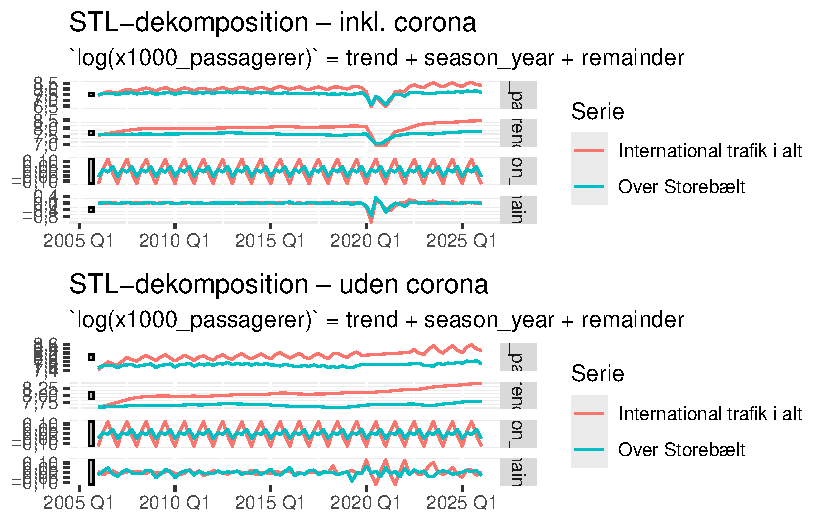
\includegraphics[keepaspectratio]{forecast_files/figure-pdf/fig-stl-panel-inkl-1.pdf}}

}

\caption{\label{fig-stl-panel-inkl}STL-dekomposition -- inkl. corona
(log-skala)}

\end{figure}%

STL dekompositioner identificerer trend, sæson og remainder for begge
serier. Trendkomponenten viser stabil vækst i international trafik frem
til 2019 med et markant dyk i 2020 (corona). Over storebælt har en mere
jævn trend med mindre udsving. Sæsonkomponenten er periodisk og stabil
for begge serier, hvilket er særlig tydeligt for international trafik.
Remainder komponenten afslører coronaperioden som et klart ikke sæsonalt
strukturbrud, som er mest markant i 2020 Q2 og understøtter konstruktion
af det interpolerede datasæt.

\begin{Shaded}
\begin{Highlighting}[]
\NormalTok{model\_jernbane }\OtherTok{\textless{}{-}} \ControlFlowTok{function}\NormalTok{(data) \{}
\NormalTok{  data }\SpecialCharTok{\%\textgreater{}\%}
    \FunctionTok{model}\NormalTok{(}
      \AttributeTok{STL =} \FunctionTok{STL}\NormalTok{(}\FunctionTok{log}\NormalTok{(x1000\_passagerer) }\SpecialCharTok{\textasciitilde{}} \FunctionTok{trend}\NormalTok{(}\AttributeTok{window =} \DecValTok{7}\NormalTok{) }\SpecialCharTok{+} \FunctionTok{season}\NormalTok{(}\AttributeTok{window =} \StringTok{"periodic"}\NormalTok{),}
                \AttributeTok{robust =} \ConstantTok{TRUE}\NormalTok{)}
\NormalTok{    ) }\SpecialCharTok{\%\textgreater{}\%}
    \FunctionTok{augment}\NormalTok{()}
\NormalTok{\}}
\end{Highlighting}
\end{Shaded}

\begin{Shaded}
\begin{Highlighting}[]
\NormalTok{kør}\FunctionTok{\_begge}\NormalTok{(}\ControlFlowTok{function}\NormalTok{(data, titel) \{}
  \FunctionTok{model\_jernbane}\NormalTok{(data) }\SpecialCharTok{\%\textgreater{}\%}
    \FunctionTok{autoplot}\NormalTok{(.resid) }\SpecialCharTok{+}
    \FunctionTok{labs}\NormalTok{(}\AttributeTok{title =} \FunctionTok{paste0}\NormalTok{(}\StringTok{"Residualer STL – "}\NormalTok{, titel),}
         \AttributeTok{y     =} \StringTok{"Residualer"}\NormalTok{,}
         \AttributeTok{x     =} \ConstantTok{NULL}\NormalTok{)}
\NormalTok{\})}
\end{Highlighting}
\end{Shaded}

\begin{figure}[H]

\centering{

\pandocbounded{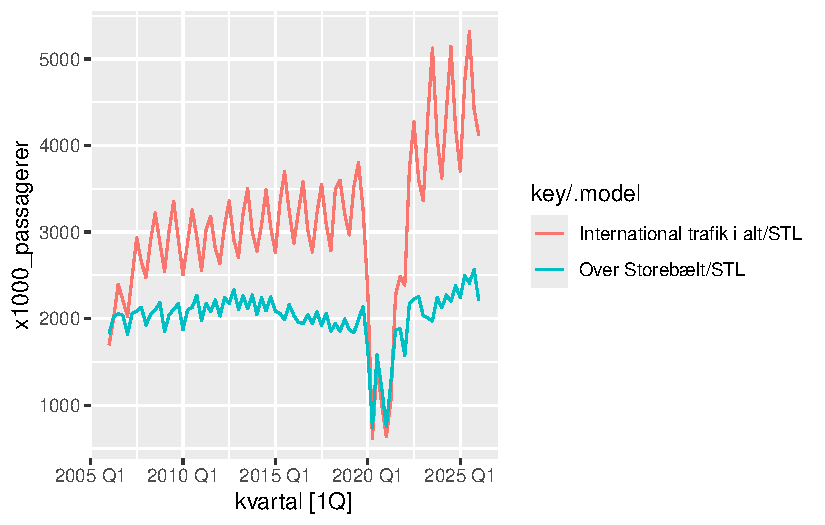
\includegraphics[keepaspectratio]{forecast_files/figure-pdf/fig-augment-inkl-1.pdf}}

}

\caption{\label{fig-augment-inkl}Fittede værdier og residualer (STL) --
inkl. corona}

\end{figure}%

Residualerne er generelt små og centrerede omkring nul, bortset fra
coronaperioden i 2020. Det store udsving i 2020 bekræfter at
coronaperioden ikke kan forklares af den normale sæson og trendstruktur.

\section{Modellering}\label{modellering}

\subsection{Træningssplit}\label{truxe6ningssplit}

Data deles i en træningsperiode (til og med 2024 Q4) og en testperiode
(fra 2025 Q1 og frem) for både datasættet inkl. og uden corona.

\begin{Shaded}
\begin{Highlighting}[]
\NormalTok{jernbane\_train }\OtherTok{\textless{}{-}}\NormalTok{ jernbanedata }\SpecialCharTok{\%\textgreater{}\%}
  \FunctionTok{filter\_index}\NormalTok{(. }\SpecialCharTok{\textasciitilde{}} \StringTok{"2024 Q4"}\NormalTok{)}

\NormalTok{jernbane\_test }\OtherTok{\textless{}{-}}\NormalTok{ jernbanedata }\SpecialCharTok{\%\textgreater{}\%}
  \FunctionTok{filter\_index}\NormalTok{(}\StringTok{"2025 Q1"} \SpecialCharTok{\textasciitilde{}}\NormalTok{ .)}

\NormalTok{jernbane\_corona\_train }\OtherTok{\textless{}{-}}\NormalTok{ jernbanedata\_corona }\SpecialCharTok{\%\textgreater{}\%}
  \FunctionTok{filter\_index}\NormalTok{(. }\SpecialCharTok{\textasciitilde{}} \StringTok{"2024 Q4"}\NormalTok{)}

\NormalTok{jernbane\_corona\_test }\OtherTok{\textless{}{-}}\NormalTok{ jernbanedata\_corona }\SpecialCharTok{\%\textgreater{}\%}
  \FunctionTok{filter\_index}\NormalTok{(}\StringTok{"2025 Q1"} \SpecialCharTok{\textasciitilde{}}\NormalTok{ .)}
\end{Highlighting}
\end{Shaded}

\subsection{Benchmark (SNAIVE)}\label{benchmark-snaive}

\begin{Shaded}
\begin{Highlighting}[]
\NormalTok{lav\_stretch }\OtherTok{\textless{}{-}} \ControlFlowTok{function}\NormalTok{(data) \{}
\NormalTok{  data }\SpecialCharTok{\%\textgreater{}\%}
    \FunctionTok{stretch\_tsibble}\NormalTok{(}\AttributeTok{.init =} \DecValTok{32}\NormalTok{, }\AttributeTok{.step =} \DecValTok{1}\NormalTok{)}
\NormalTok{\}}
\end{Highlighting}
\end{Shaded}

Fejlmål for SNAIVE-benchmarken fremgår af Bilag B.
\textbf{?@sec-bilag-b}.

\subsection{ETS-modeller}\label{ets-modeller}

\begin{Shaded}
\begin{Highlighting}[]
\NormalTok{lav\_ets }\OtherTok{\textless{}{-}} \ControlFlowTok{function}\NormalTok{(data) \{}
\NormalTok{  data }\SpecialCharTok{\%\textgreater{}\%}
    \FunctionTok{model}\NormalTok{(}
      \AttributeTok{Auto =} \FunctionTok{ETS}\NormalTok{(}\FunctionTok{log}\NormalTok{(x1000\_passagerer)),}
      \AttributeTok{AAA  =} \FunctionTok{ETS}\NormalTok{(}\FunctionTok{log}\NormalTok{(x1000\_passagerer) }\SpecialCharTok{\textasciitilde{}} \FunctionTok{error}\NormalTok{(}\StringTok{"A"}\NormalTok{) }\SpecialCharTok{+} \FunctionTok{trend}\NormalTok{(}\StringTok{"A"}\NormalTok{)  }\SpecialCharTok{+} \FunctionTok{season}\NormalTok{(}\StringTok{"A"}\NormalTok{)),}
      \AttributeTok{AAdA =} \FunctionTok{ETS}\NormalTok{(}\FunctionTok{log}\NormalTok{(x1000\_passagerer) }\SpecialCharTok{\textasciitilde{}} \FunctionTok{error}\NormalTok{(}\StringTok{"A"}\NormalTok{) }\SpecialCharTok{+} \FunctionTok{trend}\NormalTok{(}\StringTok{"Ad"}\NormalTok{) }\SpecialCharTok{+} \FunctionTok{season}\NormalTok{(}\StringTok{"A"}\NormalTok{)),}
      \AttributeTok{MAM  =} \FunctionTok{ETS}\NormalTok{(}\FunctionTok{log}\NormalTok{(x1000\_passagerer) }\SpecialCharTok{\textasciitilde{}} \FunctionTok{error}\NormalTok{(}\StringTok{"M"}\NormalTok{) }\SpecialCharTok{+} \FunctionTok{trend}\NormalTok{(}\StringTok{"A"}\NormalTok{)  }\SpecialCharTok{+} \FunctionTok{season}\NormalTok{(}\StringTok{"M"}\NormalTok{))}
\NormalTok{    )}
\NormalTok{\}}

\NormalTok{fit\_ets        }\OtherTok{\textless{}{-}} \FunctionTok{lav\_ets}\NormalTok{(jernbane\_train)}
\NormalTok{fit\_ets\_corona }\OtherTok{\textless{}{-}} \FunctionTok{lav\_ets}\NormalTok{(jernbane\_corona\_train)}
\end{Highlighting}
\end{Shaded}

Ljung-Box testoutput fremgår af Bilag C. \textbf{?@sec-bilag-c}

\begin{table}

\caption{\label{tbl-ets-inkl}ETS-modelsammenligning inkl. corona (AICc)}

\centering{

\begin{Shaded}
\begin{Highlighting}[]
\FunctionTok{glance}\NormalTok{(fit\_ets) }\SpecialCharTok{\%\textgreater{}\%}
  \FunctionTok{select}\NormalTok{(key, .model, AICc, BIC) }\SpecialCharTok{\%\textgreater{}\%}
  \FunctionTok{arrange}\NormalTok{(AICc) }\SpecialCharTok{\%\textgreater{}\%}
  \FunctionTok{kbl}\NormalTok{(}\AttributeTok{digits =} \DecValTok{2}\NormalTok{, }\AttributeTok{booktabs =} \ConstantTok{TRUE}\NormalTok{) }\SpecialCharTok{\%\textgreater{}\%}
  \FunctionTok{kable\_styling}\NormalTok{(}\AttributeTok{latex\_options =} \FunctionTok{c}\NormalTok{(}\StringTok{"striped"}\NormalTok{, }\StringTok{"hold\_position"}\NormalTok{))}
\end{Highlighting}
\end{Shaded}

\centering
\begin{tabular}[t]{llrr}
\toprule
key & .model & AICc & BIC\\
\midrule
\cellcolor{gray!10}{Over Storebælt} & \cellcolor{gray!10}{Auto} & \cellcolor{gray!10}{56,13} & \cellcolor{gray!10}{70,80}\\
Over Storebælt & AAA & 61,72 & 79,97\\
\cellcolor{gray!10}{Over Storebælt} & \cellcolor{gray!10}{AAdA} & \cellcolor{gray!10}{63,98} & \cellcolor{gray!10}{83,90}\\
Over Storebælt & MAM & 66,83 & 85,08\\
\cellcolor{gray!10}{International trafik i alt} & \cellcolor{gray!10}{Auto} & \cellcolor{gray!10}{111,71} & \cellcolor{gray!10}{126,38}\\
\addlinespace
International trafik i alt & AAA & 116,58 & 134,83\\
\cellcolor{gray!10}{International trafik i alt} & \cellcolor{gray!10}{AAdA} & \cellcolor{gray!10}{119,29} & \cellcolor{gray!10}{139,22}\\
International trafik i alt & MAM & 126,46 & 144,71\\
\bottomrule
\end{tabular}

}

\end{table}%

\begin{Shaded}
\begin{Highlighting}[]
\FunctionTok{glance}\NormalTok{(fit\_ets\_corona) }\SpecialCharTok{\%\textgreater{}\%}
  \FunctionTok{select}\NormalTok{(key, .model, AIC, AICc) }\SpecialCharTok{\%\textgreater{}\%}
  \FunctionTok{arrange}\NormalTok{(AICc) }\SpecialCharTok{\%\textgreater{}\%}
  \FunctionTok{kbl}\NormalTok{(}\AttributeTok{digits =} \DecValTok{2}\NormalTok{, }\AttributeTok{booktabs =} \ConstantTok{TRUE}\NormalTok{) }\SpecialCharTok{\%\textgreater{}\%}
  \FunctionTok{kable\_styling}\NormalTok{(}\AttributeTok{latex\_options =} \FunctionTok{c}\NormalTok{(}\StringTok{"striped"}\NormalTok{, }\StringTok{"hold\_position"}\NormalTok{))}
\end{Highlighting}
\end{Shaded}

\begin{table}

\caption{\label{tbl-ets-uden}ETS-modelsammenligning uden corona (AICc)}

\centering{

\centering
\begin{tabular}[t]{llrr}
\toprule
key & .model & AIC & AICc\\
\midrule
\cellcolor{gray!10}{Over Storebælt} & \cellcolor{gray!10}{Auto} & \cellcolor{gray!10}{-157,93} & \cellcolor{gray!10}{-156,28}\\
Over Storebælt & AAA & -154,15 & -151,42\\
\cellcolor{gray!10}{Over Storebælt} & \cellcolor{gray!10}{MAM} & \cellcolor{gray!10}{-153,61} & \cellcolor{gray!10}{-150,89}\\
Over Storebælt & AAdA & -151,90 & -148,52\\
\cellcolor{gray!10}{International trafik i alt} & \cellcolor{gray!10}{Auto} & \cellcolor{gray!10}{-108,69} & \cellcolor{gray!10}{-105,30}\\
\addlinespace
International trafik i alt & AAdA & -106,16 & -102,78\\
\cellcolor{gray!10}{International trafik i alt} & \cellcolor{gray!10}{MAM} & \cellcolor{gray!10}{-98,86} & \cellcolor{gray!10}{-96,13}\\
International trafik i alt & AAA & -97,57 & -94,85\\
\bottomrule
\end{tabular}

}

\end{table}%

Auto ETS har lavest AICc i alle fire grupper og er dermed den foretrukne
model ved begge datasæt: 56,13 og 66,83 inkl. corona, -156,28 og -105,30
uden corona. To forbehold er centrale: AICc kan kun sammenlignes inden
for samme serie og datasæt (derfor er -156,28 ikke ``bedre'' end 56,13),
Her måles kun in-sample-tilpasning --- ikke forudsigelsesevne. Dette
bliver gjort på testfejlene (RMSE)

\newpage

\subsubsection{Residualanalyse -- ETS}\label{residualanalyse-ets}

\begin{Shaded}
\begin{Highlighting}[]
\ControlFlowTok{for}\NormalTok{ (serie }\ControlFlowTok{in} \FunctionTok{c}\NormalTok{(}\StringTok{"International trafik i alt"}\NormalTok{, }\StringTok{"Over Storebælt"}\NormalTok{)) \{}
  \FunctionTok{print}\NormalTok{(}
\NormalTok{    fit\_ets }\SpecialCharTok{\%\textgreater{}\%}
      \FunctionTok{filter}\NormalTok{(key }\SpecialCharTok{==}\NormalTok{ serie) }\SpecialCharTok{\%\textgreater{}\%}
      \FunctionTok{select}\NormalTok{(Auto) }\SpecialCharTok{\%\textgreater{}\%}
      \FunctionTok{gg\_tsresiduals}\NormalTok{(}\AttributeTok{lag\_max =} \DecValTok{16}\NormalTok{) }\SpecialCharTok{+}
      \FunctionTok{labs}\NormalTok{(}\AttributeTok{title =} \FunctionTok{paste0}\NormalTok{(}\StringTok{"Residualer – Auto ETS – "}\NormalTok{, serie))}
\NormalTok{  ) }\SpecialCharTok{\%\textgreater{}\%}
  \FunctionTok{cat}\NormalTok{(}\StringTok{"}\SpecialCharTok{\textbackslash{}n\textbackslash{}n}\StringTok{"}\NormalTok{)}
\NormalTok{\}}
\end{Highlighting}
\end{Shaded}

\pandocbounded{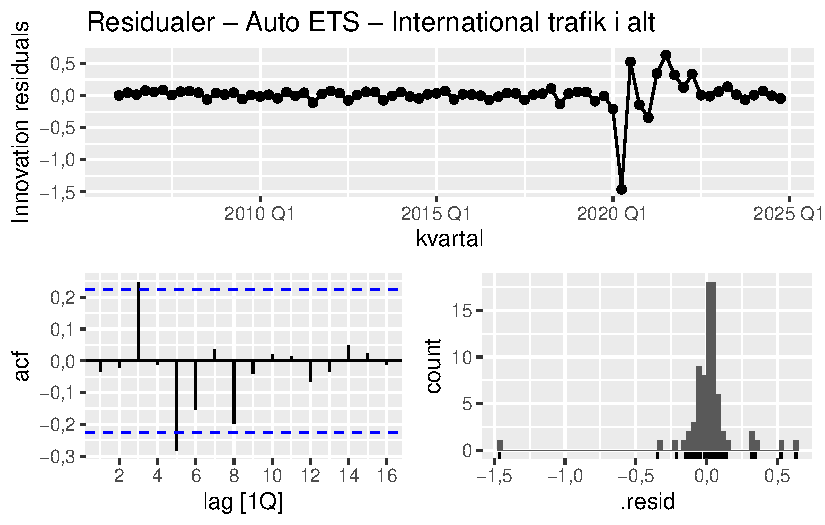
\includegraphics[keepaspectratio]{forecast_files/figure-pdf/fig-ets-residualer-inkl-1.pdf}}\pandocbounded{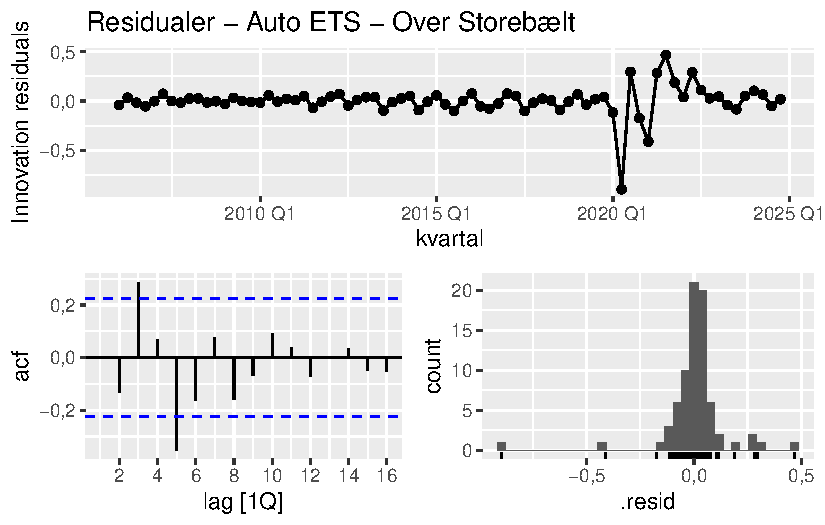
\includegraphics[keepaspectratio]{forecast_files/figure-pdf/fig-ets-residualer-inkl-2.pdf}}

Residualerne er overordnet hvid støj med et forventet udsving omkring
2020 (corona). ACF viser ingen signifikante spike og histogrammet er
tilnærmelsesvist normalfordelt. Ljung-Box testoutput fremgår af Bilag C.

\begin{Shaded}
\begin{Highlighting}[]
\ControlFlowTok{for}\NormalTok{ (serie }\ControlFlowTok{in} \FunctionTok{c}\NormalTok{(}\StringTok{"International trafik i alt"}\NormalTok{, }\StringTok{"Over Storebælt"}\NormalTok{)) \{}
  \FunctionTok{print}\NormalTok{(}
\NormalTok{    fit\_ets\_corona }\SpecialCharTok{\%\textgreater{}\%}
      \FunctionTok{filter}\NormalTok{(key }\SpecialCharTok{==}\NormalTok{ serie) }\SpecialCharTok{\%\textgreater{}\%}
      \FunctionTok{select}\NormalTok{(Auto) }\SpecialCharTok{\%\textgreater{}\%}
      \FunctionTok{gg\_tsresiduals}\NormalTok{(}\AttributeTok{lag\_max =} \DecValTok{16}\NormalTok{) }\SpecialCharTok{+}
      \FunctionTok{labs}\NormalTok{(}\AttributeTok{title =} \FunctionTok{paste0}\NormalTok{(}\StringTok{"Residualer – Auto ETS – "}\NormalTok{, serie))}
\NormalTok{  ) }\SpecialCharTok{\%\textgreater{}\%}
  \FunctionTok{cat}\NormalTok{(}\StringTok{"}\SpecialCharTok{\textbackslash{}n\textbackslash{}n}\StringTok{"}\NormalTok{)}
\NormalTok{\}}
\end{Highlighting}
\end{Shaded}

\pandocbounded{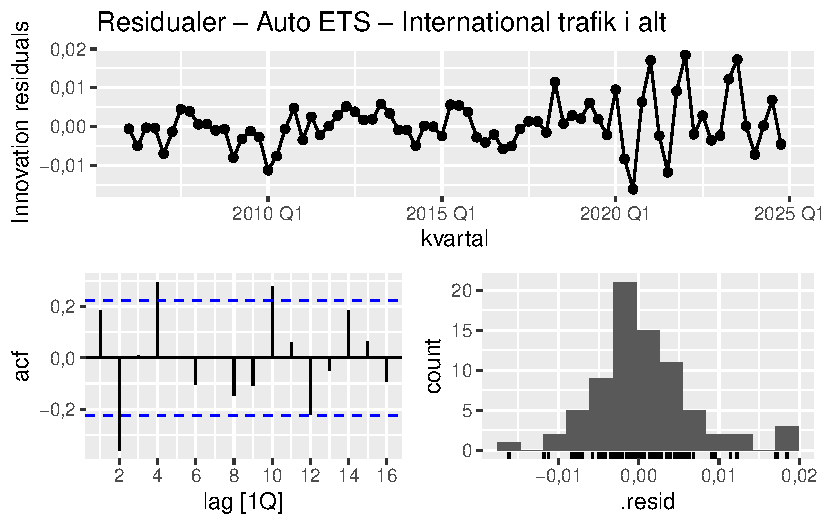
\includegraphics[keepaspectratio]{forecast_files/figure-pdf/fig-ets-residual-1.pdf}}\pandocbounded{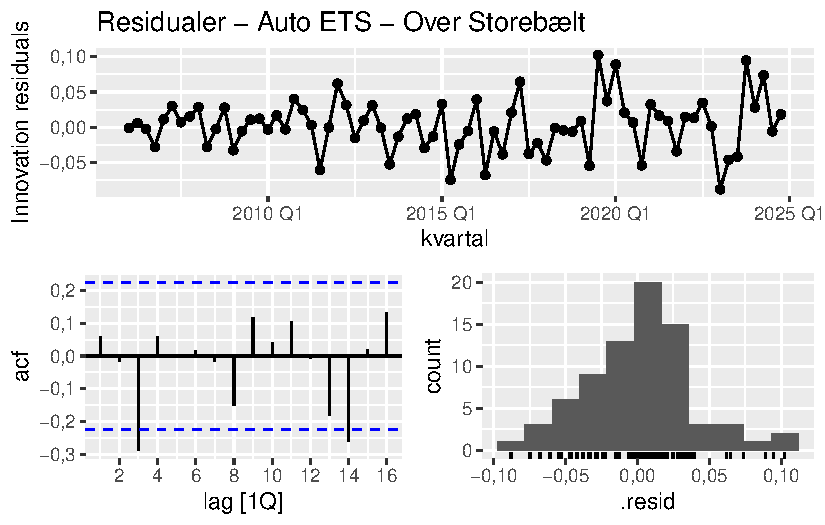
\includegraphics[keepaspectratio]{forecast_files/figure-pdf/fig-ets-residual-2.pdf}}
Residualerne ligger tæt på nul uden systematiske mønstre og ACF er inden
for konfidensintervallet. Histogrammet er tilnærmelsesvist
normalfordelt, hvilket indikerer en tilfredsstillende modeltilpasning.

Ljung-Box testen afslører en svaghed i auto ETS. inkl. corona forkastes
H0 for begge serier (international: lb = 17,2, p=0,028) hvilket
indikerer ukorrelerede residualer og ej komplet modellering af
coronadynamikken. Uden corona forbedres billedet.Storebælt passerer
testen, (lb=9,3 \& p=0,315), mens international trafik fortsat fejler
(lb=23,0 \& p=0,003). Dette er sandsynligvis grundet kompleks dynamik i
international rejseadfærd ud over coronaforstyrrelsen.

\subsection{ARIMA-modeller}\label{arima-modeller}

\begin{Shaded}
\begin{Highlighting}[]
\NormalTok{lav\_arima }\OtherTok{\textless{}{-}} \ControlFlowTok{function}\NormalTok{(data) \{}
\NormalTok{  data }\SpecialCharTok{\%\textgreater{}\%}
    \FunctionTok{model}\NormalTok{(}
      \AttributeTok{Auto =} \FunctionTok{ARIMA}\NormalTok{(}\FunctionTok{log}\NormalTok{(x1000\_passagerer)),}
      \AttributeTok{M1   =} \FunctionTok{ARIMA}\NormalTok{(}\FunctionTok{log}\NormalTok{(x1000\_passagerer) }\SpecialCharTok{\textasciitilde{}} \DecValTok{0} \SpecialCharTok{+} \FunctionTok{pdq}\NormalTok{(}\DecValTok{0}\NormalTok{,}\DecValTok{1}\NormalTok{,}\DecValTok{1}\NormalTok{) }\SpecialCharTok{+} \FunctionTok{PDQ}\NormalTok{(}\DecValTok{0}\NormalTok{,}\DecValTok{1}\NormalTok{,}\DecValTok{1}\NormalTok{)),}
      \AttributeTok{M2   =} \FunctionTok{ARIMA}\NormalTok{(}\FunctionTok{log}\NormalTok{(x1000\_passagerer) }\SpecialCharTok{\textasciitilde{}} \DecValTok{0} \SpecialCharTok{+} \FunctionTok{pdq}\NormalTok{(}\DecValTok{1}\NormalTok{,}\DecValTok{1}\NormalTok{,}\DecValTok{0}\NormalTok{) }\SpecialCharTok{+} \FunctionTok{PDQ}\NormalTok{(}\DecValTok{1}\NormalTok{,}\DecValTok{1}\NormalTok{,}\DecValTok{0}\NormalTok{)),}
      \AttributeTok{M3   =} \FunctionTok{ARIMA}\NormalTok{(}\FunctionTok{log}\NormalTok{(x1000\_passagerer) }\SpecialCharTok{\textasciitilde{}} \DecValTok{0} \SpecialCharTok{+} \FunctionTok{pdq}\NormalTok{(}\DecValTok{1}\NormalTok{,}\DecValTok{1}\NormalTok{,}\DecValTok{1}\NormalTok{) }\SpecialCharTok{+} \FunctionTok{PDQ}\NormalTok{(}\DecValTok{0}\NormalTok{,}\DecValTok{1}\NormalTok{,}\DecValTok{1}\NormalTok{)),}
      \AttributeTok{M4   =} \FunctionTok{ARIMA}\NormalTok{(}\FunctionTok{log}\NormalTok{(x1000\_passagerer) }\SpecialCharTok{\textasciitilde{}} \DecValTok{0} \SpecialCharTok{+} \FunctionTok{pdq}\NormalTok{(}\DecValTok{2}\NormalTok{,}\DecValTok{1}\NormalTok{,}\DecValTok{0}\NormalTok{) }\SpecialCharTok{+} \FunctionTok{PDQ}\NormalTok{(}\DecValTok{0}\NormalTok{,}\DecValTok{1}\NormalTok{,}\DecValTok{1}\NormalTok{))}
\NormalTok{    )}
\NormalTok{\}}

\NormalTok{fit\_arima        }\OtherTok{\textless{}{-}} \FunctionTok{lav\_arima}\NormalTok{(jernbane\_train)}
\NormalTok{fit\_arima\_corona }\OtherTok{\textless{}{-}} \FunctionTok{lav\_arima}\NormalTok{(jernbane\_corona\_train)}
\end{Highlighting}
\end{Shaded}

\begin{Shaded}
\begin{Highlighting}[]
\NormalTok{hent\_dof }\OtherTok{\textless{}{-}} \ControlFlowTok{function}\NormalTok{(fit, serie) \{}
\NormalTok{  fit }\SpecialCharTok{\%\textgreater{}\%}
    \FunctionTok{filter}\NormalTok{(key }\SpecialCharTok{==}\NormalTok{ serie) }\SpecialCharTok{\%\textgreater{}\%}
    \FunctionTok{select}\NormalTok{(Auto) }\SpecialCharTok{\%\textgreater{}\%}
    \FunctionTok{coefficients}\NormalTok{() }\SpecialCharTok{\%\textgreater{}\%}
    \FunctionTok{nrow}\NormalTok{()}
\NormalTok{\}}

\NormalTok{dof\_int }\OtherTok{\textless{}{-}} \FunctionTok{hent\_dof}\NormalTok{(fit\_arima, }\StringTok{"International trafik i alt"}\NormalTok{)}
\NormalTok{dof\_osb }\OtherTok{\textless{}{-}} \FunctionTok{hent\_dof}\NormalTok{(fit\_arima, }\StringTok{"Over Storebælt"}\NormalTok{)}

\NormalTok{dof\_int\_corona }\OtherTok{\textless{}{-}} \FunctionTok{hent\_dof}\NormalTok{(fit\_arima\_corona, }\StringTok{"International trafik i alt"}\NormalTok{)}
\NormalTok{dof\_osb\_corona }\OtherTok{\textless{}{-}} \FunctionTok{hent\_dof}\NormalTok{(fit\_arima\_corona, }\StringTok{"Over Storebælt"}\NormalTok{)}
\end{Highlighting}
\end{Shaded}

\begin{Shaded}
\begin{Highlighting}[]
\FunctionTok{glance}\NormalTok{(fit\_arima) }\SpecialCharTok{\%\textgreater{}\%}
  \FunctionTok{select}\NormalTok{(key, .model, log\_lik, AIC, AICc, BIC) }\SpecialCharTok{\%\textgreater{}\%}
  \FunctionTok{arrange}\NormalTok{(key, AICc) }\SpecialCharTok{\%\textgreater{}\%}
  \FunctionTok{kbl}\NormalTok{(}\AttributeTok{digits =} \DecValTok{2}\NormalTok{, }\AttributeTok{booktabs =} \ConstantTok{TRUE}\NormalTok{) }\SpecialCharTok{\%\textgreater{}\%}
  \FunctionTok{kable\_styling}\NormalTok{(}\AttributeTok{latex\_options =} \FunctionTok{c}\NormalTok{(}\StringTok{"striped"}\NormalTok{, }\StringTok{"hold\_position"}\NormalTok{))}
\end{Highlighting}
\end{Shaded}

\begin{table}

\caption{\label{tbl-arima-inkl}ARIMA-modelsammenligning inkl. corona
(AICc)}

\centering{

\centering
\begin{tabular}[t]{llrrrr}
\toprule
key & .model & log\_lik & AIC & AICc & BIC\\
\midrule
\cellcolor{gray!10}{International trafik i alt} & \cellcolor{gray!10}{Auto} & \cellcolor{gray!10}{1,58} & \cellcolor{gray!10}{4,85} & \cellcolor{gray!10}{5,41} & \cellcolor{gray!10}{14,17}\\
International trafik i alt & M1 & 0,01 & 5,97 & 6,33 & 12,76\\
\cellcolor{gray!10}{International trafik i alt} & \cellcolor{gray!10}{M4} & \cellcolor{gray!10}{0,13} & \cellcolor{gray!10}{7,75} & \cellcolor{gray!10}{8,36} & \cellcolor{gray!10}{16,80}\\
International trafik i alt & M3 & 0,02 & 7,96 & 8,57 & 17,01\\
\cellcolor{gray!10}{International trafik i alt} & \cellcolor{gray!10}{M2} & \cellcolor{gray!10}{-12,89} & \cellcolor{gray!10}{31,78} & \cellcolor{gray!10}{32,13} & \cellcolor{gray!10}{38,56}\\
\addlinespace
Over Storebælt & Auto & 34,16 & -60,33 & -59,77 & -51,01\\
\cellcolor{gray!10}{Over Storebælt} & \cellcolor{gray!10}{M4} & \cellcolor{gray!10}{28,90} & \cellcolor{gray!10}{-49,79} & \cellcolor{gray!10}{-49,19} & \cellcolor{gray!10}{-40,74}\\
Over Storebælt & M1 & 25,68 & -45,35 & -45,00 & -38,57\\
\cellcolor{gray!10}{Over Storebælt} & \cellcolor{gray!10}{M3} & \cellcolor{gray!10}{25,68} & \cellcolor{gray!10}{-43,37} & \cellcolor{gray!10}{-42,76} & \cellcolor{gray!10}{-34,32}\\
Over Storebælt & M2 & 13,47 & -20,94 & -20,58 & -14,15\\
\bottomrule
\end{tabular}

}

\end{table}%

\begin{Shaded}
\begin{Highlighting}[]
\FunctionTok{glance}\NormalTok{(fit\_arima\_corona) }\SpecialCharTok{\%\textgreater{}\%}
  \FunctionTok{select}\NormalTok{(key, .model, log\_lik, AIC, AICc, BIC) }\SpecialCharTok{\%\textgreater{}\%}
  \FunctionTok{arrange}\NormalTok{(key, AICc) }\SpecialCharTok{\%\textgreater{}\%}
  \FunctionTok{kbl}\NormalTok{(}\AttributeTok{digits =} \DecValTok{2}\NormalTok{, }\AttributeTok{booktabs =} \ConstantTok{TRUE}\NormalTok{) }\SpecialCharTok{\%\textgreater{}\%}
  \FunctionTok{kable\_styling}\NormalTok{(}\AttributeTok{latex\_options =} \FunctionTok{c}\NormalTok{(}\StringTok{"striped"}\NormalTok{, }\StringTok{"hold\_position"}\NormalTok{))}
\end{Highlighting}
\end{Shaded}

\begin{table}

\caption{\label{tbl-arima-uden}ARIMA-modelsammenligning uden corona
(AICc)}

\centering{

\centering
\begin{tabular}[t]{llrrrr}
\toprule
key & .model & log\_lik & AIC & AICc & BIC\\
\midrule
\cellcolor{gray!10}{International trafik i alt} & \cellcolor{gray!10}{M4} & \cellcolor{gray!10}{109,59} & \cellcolor{gray!10}{-211,17} & \cellcolor{gray!10}{-210,57} & \cellcolor{gray!10}{-202,12}\\
International trafik i alt & Auto & 106,93 & -207,87 & -207,51 & -201,04\\
\cellcolor{gray!10}{International trafik i alt} & \cellcolor{gray!10}{M3} & \cellcolor{gray!10}{103,94} & \cellcolor{gray!10}{-199,87} & \cellcolor{gray!10}{-199,27} & \cellcolor{gray!10}{-190,82}\\
International trafik i alt & M1 & 102,17 & -198,33 & -197,97 & -191,54\\
\cellcolor{gray!10}{International trafik i alt} & \cellcolor{gray!10}{M2} & \cellcolor{gray!10}{99,12} & \cellcolor{gray!10}{-192,24} & \cellcolor{gray!10}{-191,88} & \cellcolor{gray!10}{-185,45}\\
\addlinespace
Over Storebælt & Auto & 135,66 & -263,32 & -262,73 & -254,22\\
\cellcolor{gray!10}{Over Storebælt} & \cellcolor{gray!10}{M3} & \cellcolor{gray!10}{130,23} & \cellcolor{gray!10}{-252,46} & \cellcolor{gray!10}{-251,85} & \cellcolor{gray!10}{-243,41}\\
Over Storebælt & M1 & 128,83 & -251,66 & -251,30 & -244,87\\
\cellcolor{gray!10}{Over Storebælt} & \cellcolor{gray!10}{M4} & \cellcolor{gray!10}{128,74} & \cellcolor{gray!10}{-249,48} & \cellcolor{gray!10}{-248,87} & \cellcolor{gray!10}{-240,43}\\
Over Storebælt & M2 & 124,99 & -243,99 & -243,63 & -237,20\\
\bottomrule
\end{tabular}

}

\end{table}%

Inkl. corona vælger auto ARIMA: ARIMA(1,0,0)(1,0,0){[}4{]} for
international trafik (AICc = 5,41), og ARIMA(1,0,0)(0,0,1){[}4{]} for
storebælt (AICc = -59,8). Begge stationære (d=D=0), som er konsistent
med stationaritetstestene. For international trafik indikerer φ₁=0,734
(autoregressiv koeffecient) stærk AR persistens \& Φ₁ = 0,299 moderat
sæsonel persistens. For storebælt estimeres φ₁=0,518 \& Θ₁ = 0,306. Auto
udkonkurrer alle de manuelle kandidater på inkl. coronadata.
airline-modellen M1 = ARIMA(0,1,1)(0,1,1){[}4{]} scorer AICc = 6,33 ---
marginalt over Auto men er analytisk velbegrundet. Uden corona vælger
auto ARIMA: ARIMA(0,0,1)(0,1,0){[}4{]} med drift (international) og
ARIMA(1,0,0)(0,1,2){[}4{]} (Storebælt). Begge med D=1, konsistent med en
tydeligere sæsontrend.

\subsubsection{Residualanalyse -- ARIMA}\label{residualanalyse-arima}

\begin{Shaded}
\begin{Highlighting}[]
\ControlFlowTok{for}\NormalTok{ (serie }\ControlFlowTok{in} \FunctionTok{c}\NormalTok{(}\StringTok{"International trafik i alt"}\NormalTok{, }\StringTok{"Over Storebælt"}\NormalTok{)) \{}
\NormalTok{  residualer }\OtherTok{\textless{}{-}}\NormalTok{ fit\_arima }\SpecialCharTok{\%\textgreater{}\%}
    \FunctionTok{filter}\NormalTok{(key }\SpecialCharTok{==}\NormalTok{ serie) }\SpecialCharTok{\%\textgreater{}\%}
    \FunctionTok{select}\NormalTok{(Auto) }\SpecialCharTok{\%\textgreater{}\%}
    \FunctionTok{gg\_tsresiduals}\NormalTok{(}\AttributeTok{lag\_max =} \DecValTok{16}\NormalTok{) }\SpecialCharTok{+}
    \FunctionTok{labs}\NormalTok{(}\AttributeTok{title =} \FunctionTok{paste0}\NormalTok{(}\StringTok{"Residualer – Auto ARIMA – "}\NormalTok{, serie, }\StringTok{" – Inkl. corona"}\NormalTok{))}
  \FunctionTok{print}\NormalTok{(residualer)}
  \FunctionTok{cat}\NormalTok{(}\StringTok{"}\SpecialCharTok{\textbackslash{}n\textbackslash{}n}\StringTok{"}\NormalTok{)}
\NormalTok{\}}
\end{Highlighting}
\end{Shaded}

\pandocbounded{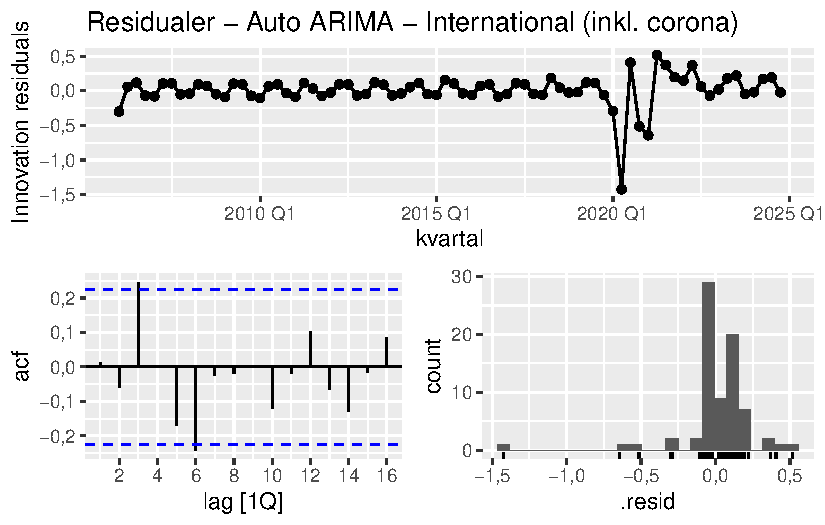
\includegraphics[keepaspectratio]{forecast_files/figure-pdf/fig-arima-res-int-inkl-1.pdf}}\pandocbounded{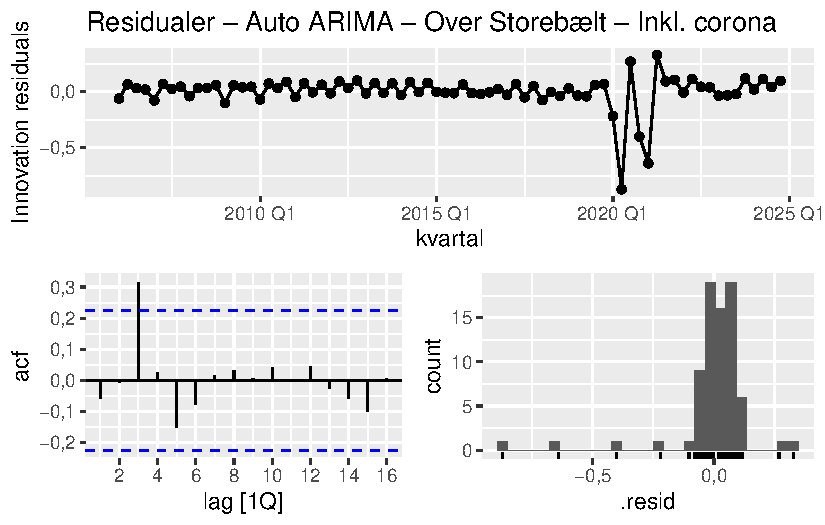
\includegraphics[keepaspectratio]{forecast_files/figure-pdf/fig-arima-res-int-inkl-2.pdf}}

\#\#\#\#International trafik i alt Residualerne er overordnet hvid støj,
men med et kraftigt coronaudsving i 2020 der skævvrider histogrammet.
ACF viser ingen signifikante spike.

\#\#\#\#Over Storbælt Residualerne er centrerede omkring nul med et
markant dyk i 2020, der ligeledes skævvrider histogrammet. ACF er inden
for konfidensintervallet på alle lags.

\begin{Shaded}
\begin{Highlighting}[]
\ControlFlowTok{for}\NormalTok{ (serie }\ControlFlowTok{in} \FunctionTok{c}\NormalTok{(}\StringTok{"International trafik i alt"}\NormalTok{, }\StringTok{"Over Storebælt"}\NormalTok{)) \{}
\NormalTok{  residualer }\OtherTok{\textless{}{-}}\NormalTok{ fit\_arima\_corona }\SpecialCharTok{\%\textgreater{}\%}
    \FunctionTok{filter}\NormalTok{(key }\SpecialCharTok{==}\NormalTok{ serie) }\SpecialCharTok{\%\textgreater{}\%}
    \FunctionTok{select}\NormalTok{(Auto) }\SpecialCharTok{\%\textgreater{}\%}
    \FunctionTok{gg\_tsresiduals}\NormalTok{(}\AttributeTok{lag\_max =} \DecValTok{16}\NormalTok{) }\SpecialCharTok{+}
    \FunctionTok{labs}\NormalTok{(}\AttributeTok{title =} \FunctionTok{paste0}\NormalTok{(}\StringTok{"Residualer – Auto ARIMA – "}\NormalTok{, serie, }\StringTok{" – Inkl. corona"}\NormalTok{))}
  \FunctionTok{print}\NormalTok{(residualer)}
  \FunctionTok{cat}\NormalTok{(}\StringTok{"}\SpecialCharTok{\textbackslash{}n\textbackslash{}n}\StringTok{"}\NormalTok{)}
\NormalTok{\}}
\end{Highlighting}
\end{Shaded}

\pandocbounded{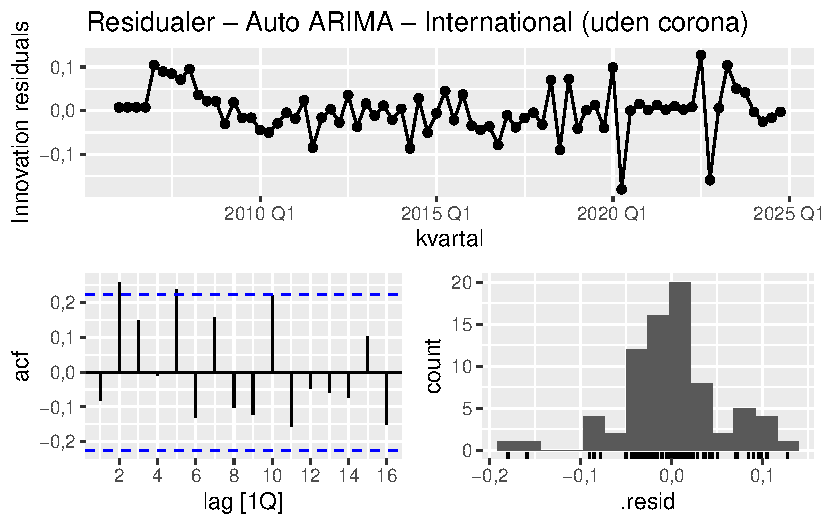
\includegraphics[keepaspectratio]{forecast_files/figure-pdf/fig-arima-res-int-uden-1.pdf}}\pandocbounded{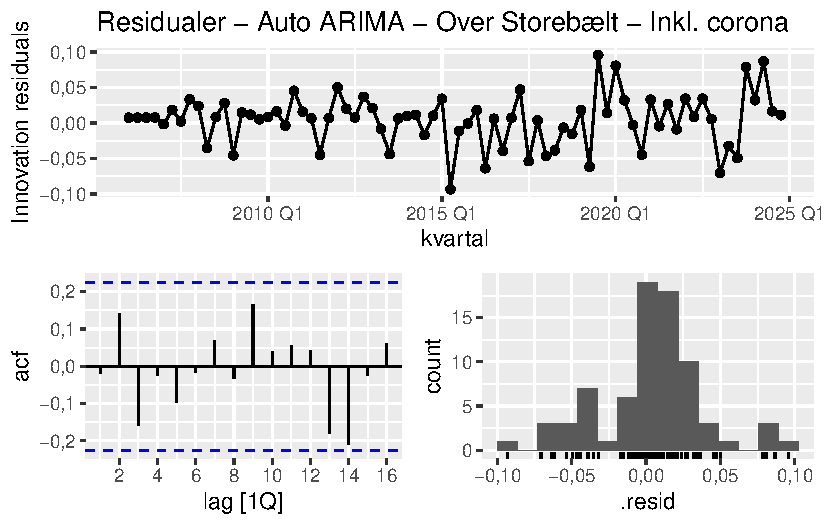
\includegraphics[keepaspectratio]{forecast_files/figure-pdf/fig-arima-res-int-uden-2.pdf}}

ARIMA residualerne er delvist bedre end ETS. For storebælt er
residualerne marginalt ikke signifikante inkl. corona (lb=11,0 \&
p=0,052) og klart white noise uden corona (lb=5,1 \& p=0,401). For
international trafik forkastes H0, i begge datasæt (p = 0,027 inkl.; p =
0,009 ekskl. corona), da det er identisk med ETS resultatet. Dette
indikerer en dynamik som ikke indfanges af hverken ETS eller ARIMA.
sandsynligvis relateret til coronaforløbet og efterfølgende
genopretningsdynamikker. Forecasts for international trafik bør derfor
tolkes med ekstra forsigtighed og brede prædiktionsintervaller.

\subsubsection{Optimal ARIMA-søgning}\label{optimal-arima-suxf8gning}

\begin{Shaded}
\begin{Highlighting}[]
\NormalTok{lav\_arima\_optimal }\OtherTok{\textless{}{-}} \ControlFlowTok{function}\NormalTok{(data) \{}
\NormalTok{  data }\SpecialCharTok{\%\textgreater{}\%}
    \FunctionTok{model}\NormalTok{(}
      \AttributeTok{Auto    =} \FunctionTok{ARIMA}\NormalTok{(}\FunctionTok{log}\NormalTok{(x1000\_passagerer)),}
      \AttributeTok{Optimal =} \FunctionTok{ARIMA}\NormalTok{(}
        \FunctionTok{log}\NormalTok{(x1000\_passagerer),}
        \AttributeTok{stepwise         =} \ConstantTok{FALSE}\NormalTok{,}
        \AttributeTok{approximation    =} \ConstantTok{FALSE}\NormalTok{,}
        \AttributeTok{order\_constraint =}\NormalTok{ p }\SpecialCharTok{+}\NormalTok{ q }\SpecialCharTok{+}\NormalTok{ P }\SpecialCharTok{+}\NormalTok{ Q }\SpecialCharTok{\textless{}=} \DecValTok{9} \SpecialCharTok{\&}\NormalTok{ (constant }\SpecialCharTok{+}\NormalTok{ d }\SpecialCharTok{+}\NormalTok{ D }\SpecialCharTok{\textless{}=} \DecValTok{2}\NormalTok{)}
\NormalTok{      )}
\NormalTok{    )}
\NormalTok{\}}

\NormalTok{fit\_arima\_optimal        }\OtherTok{\textless{}{-}} \FunctionTok{lav\_arima\_optimal}\NormalTok{(jernbane\_train)}
\NormalTok{fit\_arima\_optimal\_corona }\OtherTok{\textless{}{-}} \FunctionTok{lav\_arima\_optimal}\NormalTok{(jernbane\_corona\_train)}
\end{Highlighting}
\end{Shaded}

\begin{table}

\caption{\label{tbl-arima-optimal-inkl}Optimal ARIMA vs.~Auto -- inkl.
corona (AICc)}

\centering{

\begin{Shaded}
\begin{Highlighting}[]
\ControlFlowTok{for}\NormalTok{ (fit }\ControlFlowTok{in} \FunctionTok{list}\NormalTok{(fit\_arima\_optimal, fit\_arima\_optimal\_corona)) \{}
\NormalTok{  titel }\OtherTok{\textless{}{-}} \ControlFlowTok{if}\NormalTok{ (}\FunctionTok{identical}\NormalTok{(fit, fit\_arima\_optimal)) }\StringTok{"Inkl. corona"} \ControlFlowTok{else} \StringTok{"Uden corona"}
  \FunctionTok{glance}\NormalTok{(fit) }\SpecialCharTok{\%\textgreater{}\%}
    \FunctionTok{select}\NormalTok{(key, .model, AIC, AICc) }\SpecialCharTok{\%\textgreater{}\%}
    \FunctionTok{arrange}\NormalTok{(key, AICc) }\SpecialCharTok{\%\textgreater{}\%}
    \FunctionTok{kbl}\NormalTok{(}\AttributeTok{digits =} \DecValTok{2}\NormalTok{, }\AttributeTok{booktabs =} \ConstantTok{TRUE}\NormalTok{) }\SpecialCharTok{\%\textgreater{}\%}
    \FunctionTok{kable\_styling}\NormalTok{(}\AttributeTok{latex\_options =} \FunctionTok{c}\NormalTok{(}\StringTok{"striped"}\NormalTok{, }\StringTok{"hold\_position"}\NormalTok{)) }\SpecialCharTok{\%\textgreater{}\%}
    \FunctionTok{print}\NormalTok{()}
  \FunctionTok{cat}\NormalTok{(}\StringTok{"}\SpecialCharTok{\textbackslash{}n\textbackslash{}n}\StringTok{"}\NormalTok{)}
\NormalTok{\}}
\end{Highlighting}
\end{Shaded}

\centering
\begin{tabular}[t]{llrr}
\toprule
key & .model & AIC & AICc\\
\midrule
\cellcolor{gray!10}{International trafik i alt} & \cellcolor{gray!10}{Optimal} & \cellcolor{gray!10}{-6,90} & \cellcolor{gray!10}{-4,75}\\
International trafik i alt & Auto & 4,85 & 5,41\\
\cellcolor{gray!10}{Over Storebælt} & \cellcolor{gray!10}{Optimal} & \cellcolor{gray!10}{-76,77} & \cellcolor{gray!10}{-75,12}\\
Over Storebælt & Auto & -60,33 & -59,77\\
\bottomrule
\end{tabular}

\centering
\begin{tabular}[t]{llrr}
\toprule
key & .model & AIC & AICc\\
\midrule
\cellcolor{gray!10}{International trafik i alt} & \cellcolor{gray!10}{Optimal} & \cellcolor{gray!10}{-219,41} & \cellcolor{gray!10}{-216,50}\\
International trafik i alt & Auto & -207,87 & -207,51\\
\cellcolor{gray!10}{Over Storebælt} & \cellcolor{gray!10}{Optimal} & \cellcolor{gray!10}{-264,31} & \cellcolor{gray!10}{-263,02}\\
Over Storebælt & Auto & -263,32 & -262,73\\
\bottomrule
\end{tabular}

}

\end{table}%

Den exhaustive søgning forbedrer AICc i alle tilfælde. Inkl. Corona:
International trafik fra 5,41 til -4,75 (-10,2 enheder) \& Storebælt fra
-59,8 til -75,1 (-15,3 enheder). Uden Corona er forbedringen for
international trafik mere beskeden (-207,5 til -216,5), mens storebælt
er nærmest identisk (ca -262,7), hvilket indikerer at auto allerede
finder det globale optimum. Resultaterne bekræfter at stepwise søgning
ikke altid er tilstrækkeligt på komplekse datasæt med corona
forstyrrelser.

\section{Modelsammenligning}\label{modelsammenligning}

\begin{Shaded}
\begin{Highlighting}[]
\NormalTok{resultat }\OtherTok{\textless{}{-}} \FunctionTok{bind\_rows}\NormalTok{(}
\NormalTok{  fit\_arima }\SpecialCharTok{\%\textgreater{}\%} 
    \FunctionTok{accuracy}\NormalTok{() }\SpecialCharTok{\%\textgreater{}\%}
    \FunctionTok{mutate}\NormalTok{(}\AttributeTok{data =} \StringTok{"Inkl. corona"}\NormalTok{, }\AttributeTok{familie =} \StringTok{"ARIMA"}\NormalTok{),}
\NormalTok{  fit\_ets }\SpecialCharTok{\%\textgreater{}\%} 
    \FunctionTok{accuracy}\NormalTok{() }\SpecialCharTok{\%\textgreater{}\%} 
    \FunctionTok{mutate}\NormalTok{(}\AttributeTok{data =} \StringTok{"Inkl. corona"}\NormalTok{, }\AttributeTok{familie =} \StringTok{"ETS"}\NormalTok{),}
\NormalTok{  fit\_arima\_corona }\SpecialCharTok{\%\textgreater{}\%} 
    \FunctionTok{accuracy}\NormalTok{() }\SpecialCharTok{\%\textgreater{}\%} 
    \FunctionTok{mutate}\NormalTok{(}\AttributeTok{data =} \StringTok{"Uden corona"}\NormalTok{, }\AttributeTok{familie =} \StringTok{"ARIMA"}\NormalTok{),}
\NormalTok{  fit\_ets\_corona}\SpecialCharTok{\%\textgreater{}\%} 
    \FunctionTok{accuracy}\NormalTok{() }\SpecialCharTok{\%\textgreater{}\%} 
    \FunctionTok{mutate}\NormalTok{(}\AttributeTok{data =} \StringTok{"Uden corona"}\NormalTok{, }\AttributeTok{familie =} \StringTok{"ETS"}\NormalTok{),}
  
\NormalTok{  fit\_arima }\SpecialCharTok{\%\textgreater{}\%} 
    \FunctionTok{forecast}\NormalTok{(}\AttributeTok{h =} \DecValTok{4}\NormalTok{) }\SpecialCharTok{\%\textgreater{}\%} 
    \FunctionTok{accuracy}\NormalTok{(jernbane\_test) }\SpecialCharTok{\%\textgreater{}\%} 
    \FunctionTok{mutate}\NormalTok{(}\AttributeTok{data =} \StringTok{"Inkl. corona"}\NormalTok{, }\AttributeTok{familie =} \StringTok{"ARIMA"}\NormalTok{),}
\NormalTok{  fit\_ets }\SpecialCharTok{\%\textgreater{}\%} 
    \FunctionTok{forecast}\NormalTok{(}\AttributeTok{h =} \DecValTok{4}\NormalTok{) }\SpecialCharTok{\%\textgreater{}\%} 
    \FunctionTok{accuracy}\NormalTok{(jernbane\_test) }\SpecialCharTok{\%\textgreater{}\%} 
    \FunctionTok{mutate}\NormalTok{(}\AttributeTok{data =} \StringTok{"Inkl. corona"}\NormalTok{, }\AttributeTok{familie =} \StringTok{"ETS"}\NormalTok{),}
\NormalTok{  fit\_arima\_corona }\SpecialCharTok{\%\textgreater{}\%} 
    \FunctionTok{forecast}\NormalTok{(}\AttributeTok{h =} \DecValTok{4}\NormalTok{) }\SpecialCharTok{\%\textgreater{}\%} 
    \FunctionTok{accuracy}\NormalTok{(jernbane\_corona\_test) }\SpecialCharTok{\%\textgreater{}\%} 
    \FunctionTok{mutate}\NormalTok{(}\AttributeTok{data =} \StringTok{"Uden corona"}\NormalTok{,  }\AttributeTok{familie =} \StringTok{"ARIMA"}\NormalTok{),}
\NormalTok{  fit\_ets\_corona }\SpecialCharTok{\%\textgreater{}\%} 
    \FunctionTok{forecast}\NormalTok{(}\AttributeTok{h =} \DecValTok{4}\NormalTok{) }\SpecialCharTok{\%\textgreater{}\%} 
    \FunctionTok{accuracy}\NormalTok{(jernbane\_corona\_test) }\SpecialCharTok{\%\textgreater{}\%} 
    \FunctionTok{mutate}\NormalTok{(}\AttributeTok{data =} \StringTok{"Uden corona"}\NormalTok{,  }\AttributeTok{familie =} \StringTok{"ETS"}\NormalTok{)}
\NormalTok{) }\SpecialCharTok{\%\textgreater{}\%}
  \FunctionTok{mutate}\NormalTok{(}\FunctionTok{across}\NormalTok{(}\FunctionTok{where}\NormalTok{(is.numeric), }\SpecialCharTok{\textasciitilde{}} \FunctionTok{round}\NormalTok{(.x, }\DecValTok{2}\NormalTok{)))}
\end{Highlighting}
\end{Shaded}

Tabellerne A-H viser fejlmål opdelt på modeltype, datasæt og split, hvor
en MASE under 1 indikerer, at modellen overgår SNAIVE-benchmarken og
dermed er brugbar.

\begin{Shaded}
\begin{Highlighting}[]
\NormalTok{kombinationer }\OtherTok{\textless{}{-}} \FunctionTok{expand.grid}\NormalTok{(}
  \AttributeTok{data    =} \FunctionTok{c}\NormalTok{(}\StringTok{"Inkl. corona"}\NormalTok{, }\StringTok{"Uden corona"}\NormalTok{),}
  \AttributeTok{familie =} \FunctionTok{c}\NormalTok{(}\StringTok{"ARIMA"}\NormalTok{, }\StringTok{"ETS"}\NormalTok{),}
  \AttributeTok{type    =} \FunctionTok{c}\NormalTok{(}\StringTok{"Training"}\NormalTok{, }\StringTok{"Test"}\NormalTok{),}
  \AttributeTok{stringsAsFactors =} \ConstantTok{FALSE}
\NormalTok{)}

\NormalTok{tabel\_labels }\OtherTok{\textless{}{-}} \FunctionTok{c}\NormalTok{(}\StringTok{"A"}\NormalTok{, }\StringTok{"B"}\NormalTok{, }\StringTok{"C"}\NormalTok{, }\StringTok{"D"}\NormalTok{, }\StringTok{"E"}\NormalTok{, }\StringTok{"F"}\NormalTok{, }\StringTok{"G"}\NormalTok{, }\StringTok{"H"}\NormalTok{)}
\end{Highlighting}
\end{Shaded}

\begin{Shaded}
\begin{Highlighting}[]
\NormalTok{cols }\OtherTok{\textless{}{-}} \FunctionTok{c}\NormalTok{(}\StringTok{".model"}\NormalTok{, }\StringTok{"key"}\NormalTok{, }\StringTok{".type"}\NormalTok{, }\StringTok{"RMSE"}\NormalTok{)}

\ControlFlowTok{for}\NormalTok{ (i }\ControlFlowTok{in} \FunctionTok{seq\_len}\NormalTok{(}\FunctionTok{nrow}\NormalTok{(kombinationer))) \{}
\NormalTok{  type\_val    }\OtherTok{\textless{}{-}}\NormalTok{ kombinationer}\SpecialCharTok{$}\NormalTok{type[i]}
\NormalTok{  familie\_val }\OtherTok{\textless{}{-}}\NormalTok{ kombinationer}\SpecialCharTok{$}\NormalTok{familie[i]}
\NormalTok{  data\_val    }\OtherTok{\textless{}{-}}\NormalTok{ kombinationer}\SpecialCharTok{$}\NormalTok{data[i]}
\NormalTok{  label       }\OtherTok{\textless{}{-}}\NormalTok{ tabel\_labels[i]}
\NormalTok{  type\_dk     }\OtherTok{\textless{}{-}} \ControlFlowTok{if}\NormalTok{ (type\_val }\SpecialCharTok{==} \StringTok{"Training"}\NormalTok{) }\StringTok{"træning"} \ControlFlowTok{else} \StringTok{"test"}
  
\NormalTok{  resultat }\SpecialCharTok{\%\textgreater{}\%}
    \FunctionTok{filter}\NormalTok{(data }\SpecialCharTok{==}\NormalTok{ data\_val,}
\NormalTok{           familie }\SpecialCharTok{==}\NormalTok{ familie\_val,}
\NormalTok{           .type }\SpecialCharTok{==}\NormalTok{ type\_val) }\SpecialCharTok{\%\textgreater{}\%}
    \FunctionTok{select}\NormalTok{(}\FunctionTok{all\_of}\NormalTok{(cols)) }\SpecialCharTok{\%\textgreater{}\%}
    \FunctionTok{arrange}\NormalTok{(key, RMSE) }\SpecialCharTok{\%\textgreater{}\%}
    \FunctionTok{kbl}\NormalTok{(}\AttributeTok{digits =} \DecValTok{2}\NormalTok{, }\AttributeTok{booktabs =} \ConstantTok{TRUE}\NormalTok{) }\SpecialCharTok{\%\textgreater{}\%}
    \FunctionTok{kable\_styling}\NormalTok{(}\AttributeTok{latex\_options =} \FunctionTok{c}\NormalTok{(}\StringTok{"striped"}\NormalTok{, }\StringTok{"hold\_position"}\NormalTok{))}
\NormalTok{\}}
\end{Highlighting}
\end{Shaded}

\texttt{slice\_min}/\texttt{slice\_max} finder den model med lavest og
højest RMSE pr. gruppe og giver et hurtigt overblik over, hvilke
modeller der konsekvent præsterer bedst.

\begin{Shaded}
\begin{Highlighting}[]
\NormalTok{opsummering }\OtherTok{\textless{}{-}}\NormalTok{ resultat }\SpecialCharTok{\%\textgreater{}\%}
  \FunctionTok{group\_by}\NormalTok{(data, familie, .type, key) }\SpecialCharTok{\%\textgreater{}\%}
  \FunctionTok{summarise}\NormalTok{(}
    \AttributeTok{Bedst\_model    =}\NormalTok{ .model[}\FunctionTok{which.min}\NormalTok{(RMSE)],}
    \AttributeTok{Bedst\_RMSE     =} \FunctionTok{min}\NormalTok{(RMSE),}
    \AttributeTok{Bedst\_MAPE     =}\NormalTok{ MAPE[}\FunctionTok{which.min}\NormalTok{(RMSE)],}
    \AttributeTok{.groups =} \StringTok{"drop"}
\NormalTok{  ) }\SpecialCharTok{\%\textgreater{}\%}
  \FunctionTok{arrange}\NormalTok{(data, .type, familie, key)}

\NormalTok{opsummering }\SpecialCharTok{\%\textgreater{}\%}
  \FunctionTok{kbl}\NormalTok{(}\AttributeTok{digits =} \DecValTok{2}\NormalTok{, }\AttributeTok{booktabs =} \ConstantTok{TRUE}\NormalTok{) }\SpecialCharTok{\%\textgreater{}\%}
  \FunctionTok{kable\_styling}\NormalTok{(}\AttributeTok{latex\_options =} \FunctionTok{c}\NormalTok{(}\StringTok{"striped"}\NormalTok{, }\StringTok{"hold\_position"}\NormalTok{))}
\end{Highlighting}
\end{Shaded}

\begin{table}

\caption{\label{tbl-opsummering}Opsummering: Bedste og dårligste model
per gruppe}

\centering{

\centering
\begin{tabular}[t]{lllllrr}
\toprule
data & familie & .type & key & Bedst\_model & Bedst\_RMSE & Bedst\_MAPE\\
\midrule
\cellcolor{gray!10}{Inkl. corona} & \cellcolor{gray!10}{ARIMA} & \cellcolor{gray!10}{Test} & \cellcolor{gray!10}{International trafik i alt} & \cellcolor{gray!10}{M4} & \cellcolor{gray!10}{259,28} & \cellcolor{gray!10}{5,16}\\
Inkl. corona & ARIMA & Test & Over Storebælt & M2 & 69,55 & 2,49\\
\cellcolor{gray!10}{Inkl. corona} & \cellcolor{gray!10}{ETS} & \cellcolor{gray!10}{Test} & \cellcolor{gray!10}{International trafik i alt} & \cellcolor{gray!10}{Auto} & \cellcolor{gray!10}{215,82} & \cellcolor{gray!10}{3,71}\\
Inkl. corona & ETS & Test & Over Storebælt & MAM & 144,39 & 4,96\\
\cellcolor{gray!10}{Inkl. corona} & \cellcolor{gray!10}{ARIMA} & \cellcolor{gray!10}{Training} & \cellcolor{gray!10}{International trafik i alt} & \cellcolor{gray!10}{M1} & \cellcolor{gray!10}{351,82} & \cellcolor{gray!10}{10,43}\\
\addlinespace
Inkl. corona & ARIMA & Training & Over Storebælt & M4 & 199,33 & 7,29\\
\cellcolor{gray!10}{Inkl. corona} & \cellcolor{gray!10}{ETS} & \cellcolor{gray!10}{Training} & \cellcolor{gray!10}{International trafik i alt} & \cellcolor{gray!10}{Auto} & \cellcolor{gray!10}{363,49} & \cellcolor{gray!10}{11,63}\\
Inkl. corona & ETS & Training & Over Storebælt & Auto & 208,10 & 8,35\\
\cellcolor{gray!10}{Uden corona} & \cellcolor{gray!10}{ARIMA} & \cellcolor{gray!10}{Test} & \cellcolor{gray!10}{International trafik i alt} & \cellcolor{gray!10}{M3} & \cellcolor{gray!10}{94,73} & \cellcolor{gray!10}{1,75}\\
Uden corona & ARIMA & Test & Over Storebælt & M2 & 121,27 & 4,25\\
\addlinespace
\cellcolor{gray!10}{Uden corona} & \cellcolor{gray!10}{ETS} & \cellcolor{gray!10}{Test} & \cellcolor{gray!10}{International trafik i alt} & \cellcolor{gray!10}{MAM} & \cellcolor{gray!10}{188,23} & \cellcolor{gray!10}{3,81}\\
Uden corona & ETS & Test & Over Storebælt & AAA & 160,92 & 5,72\\
\cellcolor{gray!10}{Uden corona} & \cellcolor{gray!10}{ARIMA} & \cellcolor{gray!10}{Training} & \cellcolor{gray!10}{International trafik i alt} & \cellcolor{gray!10}{M4} & \cellcolor{gray!10}{175,12} & \cellcolor{gray!10}{3,60}\\
Uden corona & ARIMA & Training & Over Storebælt & Auto & 73,23 & 2,65\\
\cellcolor{gray!10}{Uden corona} & \cellcolor{gray!10}{ETS} & \cellcolor{gray!10}{Training} & \cellcolor{gray!10}{International trafik i alt} & \cellcolor{gray!10}{Auto} & \cellcolor{gray!10}{178,14} & \cellcolor{gray!10}{3,51}\\
\addlinespace
Uden corona & ETS & Training & Over Storebælt & AAA & 76,60 & 2,78\\
\bottomrule
\end{tabular}

}

\end{table}%

\subsection{Time series cross
validation}\label{time-series-cross-validation}

\begin{Shaded}
\begin{Highlighting}[]
\CommentTok{\# Time series cross validation med corona}
\NormalTok{lav\_tscv }\OtherTok{\textless{}{-}} \ControlFlowTok{function}\NormalTok{(stretch, reference, data\_label) \{}
\NormalTok{  stretch }\SpecialCharTok{\%\textgreater{}\%}
    \FunctionTok{model}\NormalTok{(}
      \AttributeTok{ARIMA  =} \FunctionTok{ARIMA}\NormalTok{(}\FunctionTok{log}\NormalTok{(x1000\_passagerer)),}
      \AttributeTok{ETS    =} \FunctionTok{ETS}\NormalTok{(}\FunctionTok{log}\NormalTok{(x1000\_passagerer)),}
      \AttributeTok{SNAIVE =} \FunctionTok{SNAIVE}\NormalTok{(}\FunctionTok{log}\NormalTok{(x1000\_passagerer))}
\NormalTok{    ) }\SpecialCharTok{\%\textgreater{}\%}
    \FunctionTok{forecast}\NormalTok{(}\AttributeTok{h =} \DecValTok{3}\NormalTok{) }\SpecialCharTok{\%\textgreater{}\%}
    \FunctionTok{accuracy}\NormalTok{(reference) }\SpecialCharTok{\%\textgreater{}\%}
    \FunctionTok{mutate}\NormalTok{(}\AttributeTok{data =}\NormalTok{ data\_label)}
\NormalTok{\}}

\NormalTok{resultat\_tscv        }\OtherTok{\textless{}{-}} \FunctionTok{lav\_tscv}\NormalTok{(}\FunctionTok{lav\_stretch}\NormalTok{(jernbanedata),}
\NormalTok{                                 jernbanedata,}
                                 \StringTok{"Inkl. corona"}\NormalTok{)}
\NormalTok{resultat\_tscv\_corona }\OtherTok{\textless{}{-}} \FunctionTok{lav\_tscv}\NormalTok{(}\FunctionTok{lav\_stretch}\NormalTok{(jernbanedata\_corona), }
\NormalTok{                                 jernbanedata\_corona, }
                                 \StringTok{"Uden corona"}\NormalTok{)}
\end{Highlighting}
\end{Shaded}

\begin{Shaded}
\begin{Highlighting}[]
\FunctionTok{bind\_rows}\NormalTok{(resultat\_tscv, resultat\_tscv\_corona) }\SpecialCharTok{\%\textgreater{}\%}
  \FunctionTok{select}\NormalTok{(data, .model, key, RMSE, MAE, MAPE, MASE) }\SpecialCharTok{\%\textgreater{}\%}
  \FunctionTok{arrange}\NormalTok{(data, key, RMSE) }\SpecialCharTok{\%\textgreater{}\%}
  \FunctionTok{kbl}\NormalTok{(}\AttributeTok{digits =} \DecValTok{2}\NormalTok{, }\AttributeTok{booktabs =} \ConstantTok{TRUE}\NormalTok{) }\SpecialCharTok{\%\textgreater{}\%}
  \FunctionTok{kable\_styling}\NormalTok{(}\AttributeTok{latex\_options =} \FunctionTok{c}\NormalTok{(}\StringTok{"striped"}\NormalTok{, }\StringTok{"hold\_position"}\NormalTok{))}
\end{Highlighting}
\end{Shaded}

\begin{table}

\caption{\label{tbl-tscv}TSCV-modelsammenligning inkl. og uden corona}

\centering{

\centering
\begin{tabular}[t]{lllrrrr}
\toprule
data & .model & key & RMSE & MAE & MAPE & MASE\\
\midrule
\cellcolor{gray!10}{Inkl. corona} & \cellcolor{gray!10}{ETS} & \cellcolor{gray!10}{International trafik i alt} & \cellcolor{gray!10}{679,32} & \cellcolor{gray!10}{389,41} & \cellcolor{gray!10}{23,27} & \cellcolor{gray!10}{0,92}\\
Inkl. corona & ARIMA & International trafik i alt & 769,70 & 484,83 & 26,35 & 1,15\\
\cellcolor{gray!10}{Inkl. corona} & \cellcolor{gray!10}{SNAIVE} & \cellcolor{gray!10}{International trafik i alt} & \cellcolor{gray!10}{929,59} & \cellcolor{gray!10}{532,93} & \cellcolor{gray!10}{34,73} & \cellcolor{gray!10}{1,26}\\
Inkl. corona & SNAIVE & Over Storebælt & 360,41 & 236,66 & 16,46 & 1,37\\
\cellcolor{gray!10}{Inkl. corona} & \cellcolor{gray!10}{ETS} & \cellcolor{gray!10}{Over Storebælt} & \cellcolor{gray!10}{378,66} & \cellcolor{gray!10}{225,47} & \cellcolor{gray!10}{15,50} & \cellcolor{gray!10}{1,31}\\
\addlinespace
Inkl. corona & ARIMA & Over Storebælt & 387,45 & 253,77 & 16,59 & 1,47\\
\cellcolor{gray!10}{Uden corona} & \cellcolor{gray!10}{SNAIVE} & \cellcolor{gray!10}{International trafik i alt} & \cellcolor{gray!10}{259,98} & \cellcolor{gray!10}{191,78} & \cellcolor{gray!10}{5,09} & \cellcolor{gray!10}{1,01}\\
Uden corona & ARIMA & International trafik i alt & 270,08 & 190,71 & 5,10 & 1,00\\
\cellcolor{gray!10}{Uden corona} & \cellcolor{gray!10}{ETS} & \cellcolor{gray!10}{International trafik i alt} & \cellcolor{gray!10}{277,06} & \cellcolor{gray!10}{194,70} & \cellcolor{gray!10}{5,12} & \cellcolor{gray!10}{1,02}\\
Uden corona & ETS & Over Storebælt & 116,21 & 90,72 & 4,28 & 1,09\\
\addlinespace
\cellcolor{gray!10}{Uden corona} & \cellcolor{gray!10}{ARIMA} & \cellcolor{gray!10}{Over Storebælt} & \cellcolor{gray!10}{124,77} & \cellcolor{gray!10}{100,32} & \cellcolor{gray!10}{4,71} & \cellcolor{gray!10}{1,21}\\
Uden corona & SNAIVE & Over Storebælt & 128,76 & 100,65 & 4,73 & 1,21\\
\bottomrule
\end{tabular}

}

\end{table}%

TSCV er den metodisk mest robuste evaluering. En central begrænsning er
at ingen model opnår MASE \textless{} 1 på nogen kombination, Det er
altså ikke alle modeller der slår SNAIVE benchmark modellen. Inkl.
corona dominerer COVID kvartalerne fejlestimaterne: RMSE på 762--934
(international) og 362--409 (Storebælt), MASE på 1,04--1,55. Uden corona
er fejlene markant lavere, og MASE tættest på 1. ARIMA og SNAIVE er
næsten identiske for international trafik (MASE=1,01) mens ETS marginalt
er bedst for storebælt (RMSE = 120, MASE = 1,14). At MASE fortsat
overstiger 1 skyldes sandsynligvis, at det stærke og konsistente
sæsonmønster netop favoriserer SNAIVE. Corona perioden forringer
evalueringsgrundlaget inkl. corona kraftigt, det interpolerede datasæt
giver et mere retvisende billede af modellernes relative præstation.

\begin{Shaded}
\begin{Highlighting}[]
\NormalTok{lav\_actuals }\OtherTok{\textless{}{-}} \ControlFlowTok{function}\NormalTok{(data) \{}
\NormalTok{  data }\SpecialCharTok{\%\textgreater{}\%}
    \FunctionTok{as\_tibble}\NormalTok{() }\SpecialCharTok{\%\textgreater{}\%}
    \FunctionTok{select}\NormalTok{(kvartal, key, }\AttributeTok{actual =}\NormalTok{ x1000\_passagerer)}
\NormalTok{\}}

\NormalTok{actuals        }\OtherTok{\textless{}{-}} \FunctionTok{lav\_actuals}\NormalTok{(jernbanedata)}
\NormalTok{actuals\_corona }\OtherTok{\textless{}{-}} \FunctionTok{lav\_actuals}\NormalTok{(jernbanedata\_corona)}
\end{Highlighting}
\end{Shaded}

\begin{Shaded}
\begin{Highlighting}[]
\NormalTok{lav\_rmse\_plot }\OtherTok{\textless{}{-}} \ControlFlowTok{function}\NormalTok{(stretch, actuals\_data, titel) \{}
\NormalTok{  stretch }\SpecialCharTok{\%\textgreater{}\%}
    \FunctionTok{model}\NormalTok{(}
      \AttributeTok{ARIMA  =} \FunctionTok{ARIMA}\NormalTok{(}\FunctionTok{log}\NormalTok{(x1000\_passagerer)),}
      \AttributeTok{ETS    =} \FunctionTok{ETS}\NormalTok{(}\FunctionTok{log}\NormalTok{(x1000\_passagerer)),}
      \AttributeTok{SNAIVE =} \FunctionTok{SNAIVE}\NormalTok{(}\FunctionTok{log}\NormalTok{(x1000\_passagerer))}
\NormalTok{    ) }\SpecialCharTok{\%\textgreater{}\%}
    \FunctionTok{forecast}\NormalTok{(}\AttributeTok{h =} \DecValTok{3}\NormalTok{) }\SpecialCharTok{\%\textgreater{}\%}
    \FunctionTok{as\_tibble}\NormalTok{() }\SpecialCharTok{\%\textgreater{}\%}
    \FunctionTok{group\_by}\NormalTok{(.id, key, .model) }\SpecialCharTok{\%\textgreater{}\%}
    \FunctionTok{mutate}\NormalTok{(}\AttributeTok{h =} \FunctionTok{row\_number}\NormalTok{()) }\SpecialCharTok{\%\textgreater{}\%}
    \FunctionTok{ungroup}\NormalTok{() }\SpecialCharTok{\%\textgreater{}\%}
    \FunctionTok{left\_join}\NormalTok{(actuals\_data, }\AttributeTok{by =} \FunctionTok{c}\NormalTok{(}\StringTok{"kvartal"}\NormalTok{, }\StringTok{"key"}\NormalTok{)) }\SpecialCharTok{\%\textgreater{}\%}
    \FunctionTok{group\_by}\NormalTok{(.model, key, h) }\SpecialCharTok{\%\textgreater{}\%}
    \FunctionTok{summarise}\NormalTok{(}\AttributeTok{RMSE =} \FunctionTok{sqrt}\NormalTok{(}\FunctionTok{mean}\NormalTok{((.mean }\SpecialCharTok{{-}}\NormalTok{ actual)}\SpecialCharTok{\^{}}\DecValTok{2}\NormalTok{, }\AttributeTok{na.rm =} \ConstantTok{TRUE}\NormalTok{)),}
              \AttributeTok{.groups =} \StringTok{"drop"}\NormalTok{) }\SpecialCharTok{\%\textgreater{}\%}
    \FunctionTok{ggplot}\NormalTok{(}\FunctionTok{aes}\NormalTok{(}\AttributeTok{x =}\NormalTok{ h, }\AttributeTok{y =}\NormalTok{ RMSE, }\AttributeTok{colour =}\NormalTok{ .model)) }\SpecialCharTok{+}
    \FunctionTok{geom\_line}\NormalTok{() }\SpecialCharTok{+}
    \FunctionTok{geom\_point}\NormalTok{() }\SpecialCharTok{+}
    \FunctionTok{facet\_wrap}\NormalTok{(}\SpecialCharTok{\textasciitilde{}}\NormalTok{ key, }\AttributeTok{scales =} \StringTok{"free\_y"}\NormalTok{) }\SpecialCharTok{+}
    \FunctionTok{scale\_x\_continuous}\NormalTok{(}\AttributeTok{breaks =} \DecValTok{1}\SpecialCharTok{:}\DecValTok{3}\NormalTok{,}
                       \AttributeTok{labels =} \FunctionTok{c}\NormalTok{(}\StringTok{"Q+1"}\NormalTok{, }\StringTok{"Q+2"}\NormalTok{, }\StringTok{"Q+3"}\NormalTok{)) }\SpecialCharTok{+}
    \FunctionTok{labs}\NormalTok{(}\AttributeTok{x =} \StringTok{"Horisont"}\NormalTok{,}
         \AttributeTok{y =} \StringTok{"RMSE"}\NormalTok{,}
         \AttributeTok{colour =} \StringTok{"Model"}\NormalTok{) }\SpecialCharTok{+}
    \FunctionTok{theme\_minimal}\NormalTok{()}
\NormalTok{\}}

\NormalTok{kør}\FunctionTok{\_begge}\NormalTok{(}\ControlFlowTok{function}\NormalTok{(data, titel) \{}
\NormalTok{  stretch  }\OtherTok{\textless{}{-}} \FunctionTok{lav\_stretch}\NormalTok{(data)}
\NormalTok{  act      }\OtherTok{\textless{}{-}} \FunctionTok{lav\_actuals}\NormalTok{(data)}
  \FunctionTok{lav\_rmse\_plot}\NormalTok{(stretch, act, titel)}
\NormalTok{\})}
\end{Highlighting}
\end{Shaded}

\begin{figure}[H]

\centering{

\pandocbounded{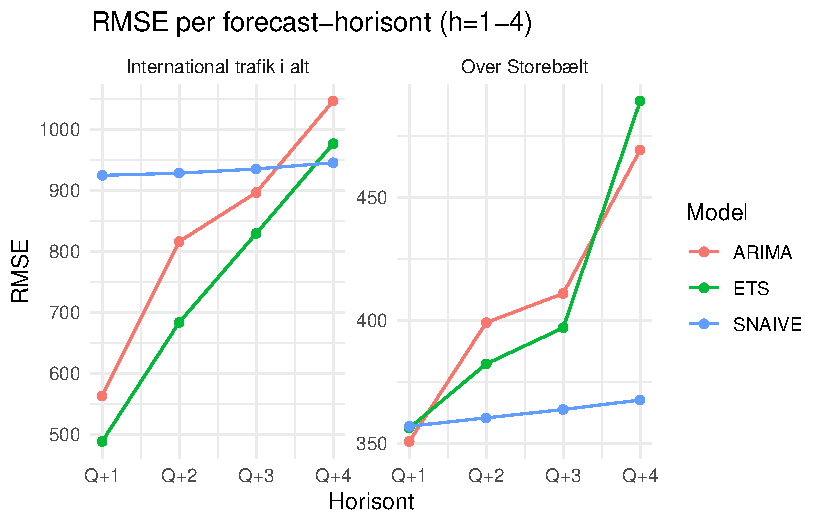
\includegraphics[keepaspectratio]{forecast_files/figure-pdf/fig-rmse-horisont-inkl-1.pdf}}

}

\caption{\label{fig-rmse-horisont-inkl}RMSE per forecast-horisont
(h=1--4)}

\end{figure}%

RMSE stiger med horisonten hvilket er forventet da usikkerheden
akkumuleres over tid. Uden corona er RMSE markant lavere og modellerne
præsterer mere stabilt på tværs af horisonterne.

\section{Forecasting og prædiktion}\label{forecasting-og-pruxe6diktion}

\begin{table}

\caption{\label{tbl-pred-uden}NULL}

\centering{

\begin{Shaded}
\begin{Highlighting}[]
\NormalTok{lav\_pred\_tbl }\OtherTok{\textless{}{-}} \ControlFlowTok{function}\NormalTok{(data, titel) \{}
\NormalTok{  data }\SpecialCharTok{\%\textgreater{}\%}
    \FunctionTok{model}\NormalTok{(}
      \AttributeTok{ARIMA =} \FunctionTok{ARIMA}\NormalTok{(}\FunctionTok{log}\NormalTok{(x1000\_passagerer)),}
      \AttributeTok{ETS   =} \FunctionTok{ETS}\NormalTok{(}\FunctionTok{log}\NormalTok{(x1000\_passagerer))}
\NormalTok{    ) }\SpecialCharTok{\%\textgreater{}\%}
    \FunctionTok{forecast}\NormalTok{(}\AttributeTok{h =} \DecValTok{3}\NormalTok{) }\SpecialCharTok{\%\textgreater{}\%}
    \FunctionTok{hilo}\NormalTok{(}\AttributeTok{level =} \FunctionTok{c}\NormalTok{(}\DecValTok{80}\NormalTok{, }\DecValTok{95}\NormalTok{)) }\SpecialCharTok{\%\textgreater{}\%}
    \FunctionTok{unpack\_hilo}\NormalTok{(}\FunctionTok{c}\NormalTok{(}\StringTok{"80\%"}\NormalTok{, }\StringTok{"95\%"}\NormalTok{)) }\SpecialCharTok{\%\textgreater{}\%}
    \FunctionTok{select}\NormalTok{(key, .model, kvartal, .mean,}
           \StringTok{\textasciigrave{}}\AttributeTok{80\%\_lower}\StringTok{\textasciigrave{}}\NormalTok{, }\StringTok{\textasciigrave{}}\AttributeTok{80\%\_upper}\StringTok{\textasciigrave{}}\NormalTok{,}
           \StringTok{\textasciigrave{}}\AttributeTok{95\%\_lower}\StringTok{\textasciigrave{}}\NormalTok{, }\StringTok{\textasciigrave{}}\AttributeTok{95\%\_upper}\StringTok{\textasciigrave{}}\NormalTok{) }\SpecialCharTok{\%\textgreater{}\%}
    \FunctionTok{as\_tibble}\NormalTok{() }\SpecialCharTok{\%\textgreater{}\%}
    \FunctionTok{kbl}\NormalTok{(}\AttributeTok{digits   =} \DecValTok{0}\NormalTok{, }\AttributeTok{booktabs =} \ConstantTok{TRUE}\NormalTok{) }\SpecialCharTok{\%\textgreater{}\%}
    \FunctionTok{kable\_styling}\NormalTok{(}\AttributeTok{latex\_options =} \FunctionTok{c}\NormalTok{(}\StringTok{"striped"}\NormalTok{, }\StringTok{"hold\_position"}\NormalTok{)) }\SpecialCharTok{\%\textgreater{}\%}
    \FunctionTok{print}\NormalTok{()}
  \FunctionTok{cat}\NormalTok{(}\StringTok{"}\SpecialCharTok{\textbackslash{}n\textbackslash{}n}\StringTok{"}\NormalTok{)}
\NormalTok{\}}

\NormalTok{kør}\FunctionTok{\_begge\_tbl}\NormalTok{(lav\_pred\_tbl)}
\end{Highlighting}
\end{Shaded}

\centering
\begin{tabular}[t]{lllrrrrr}
\toprule
key & .model & kvartal & .mean & 80\%\_lower & 80\%\_upper & 95\%\_lower & 95\%\_upper\\
\midrule
\cellcolor{gray!10}{International trafik i alt} & \cellcolor{gray!10}{ARIMA} & \cellcolor{gray!10}{2026 Q2} & \cellcolor{gray!10}{4274} & \cellcolor{gray!10}{3082} & \cellcolor{gray!10}{5615} & \cellcolor{gray!10}{2629} & \cellcolor{gray!10}{6582}\\
International trafik i alt & ARIMA & 2026 Q3 & 4266 & 2815 & 5948 & 2310 & 7250\\
\cellcolor{gray!10}{International trafik i alt} & \cellcolor{gray!10}{ARIMA} & \cellcolor{gray!10}{2026 Q4} & \cellcolor{gray!10}{3900} & \cellcolor{gray!10}{2465} & \cellcolor{gray!10}{5587} & \cellcolor{gray!10}{1984} & \cellcolor{gray!10}{6939}\\
International trafik i alt & ETS & 2026 Q2 & 4756 & 3511 & 6146 & 3027 & 7127\\
\cellcolor{gray!10}{International trafik i alt} & \cellcolor{gray!10}{ETS} & \cellcolor{gray!10}{2026 Q3} & \cellcolor{gray!10}{5664} & \cellcolor{gray!10}{3742} & \cellcolor{gray!10}{7891} & \cellcolor{gray!10}{3072} & \cellcolor{gray!10}{9613}\\
\addlinespace
International trafik i alt & ETS & 2026 Q4 & 4979 & 3001 & 7339 & 2369 & 9299\\
\cellcolor{gray!10}{Over Storebælt} & \cellcolor{gray!10}{ARIMA} & \cellcolor{gray!10}{2026 Q2} & \cellcolor{gray!10}{2284} & \cellcolor{gray!10}{1859} & \cellcolor{gray!10}{2743} & \cellcolor{gray!10}{1677} & \cellcolor{gray!10}{3041}\\
Over Storebælt & ARIMA & 2026 Q3 & 2233 & 1781 & 2724 & 1591 & 3049\\
\cellcolor{gray!10}{Over Storebælt} & \cellcolor{gray!10}{ARIMA} & \cellcolor{gray!10}{2026 Q4} & \cellcolor{gray!10}{2239} & \cellcolor{gray!10}{1767} & \cellcolor{gray!10}{2755} & \cellcolor{gray!10}{1571} & \cellcolor{gray!10}{3098}\\
Over Storebælt & ETS & 2026 Q2 & 2391 & 1946 & 2871 & 1756 & 3182\\
\addlinespace
\cellcolor{gray!10}{Over Storebælt} & \cellcolor{gray!10}{ETS} & \cellcolor{gray!10}{2026 Q3} & \cellcolor{gray!10}{2490} & \cellcolor{gray!10}{1960} & \cellcolor{gray!10}{3069} & \cellcolor{gray!10}{1740} & \cellcolor{gray!10}{3456}\\
Over Storebælt & ETS & 2026 Q4 & 2579 & 1970 & 3252 & 1725 & 3713\\
\bottomrule
\end{tabular}

NULL

\centering
\begin{tabular}[t]{lllrrrrr}
\toprule
key & .model & kvartal & .mean & 80\%\_lower & 80\%\_upper & 95\%\_lower & 95\%\_upper\\
\midrule
\cellcolor{gray!10}{International trafik i alt} & \cellcolor{gray!10}{ARIMA} & \cellcolor{gray!10}{2026 Q2} & \cellcolor{gray!10}{5034} & \cellcolor{gray!10}{4688} & \cellcolor{gray!10}{5390} & \cellcolor{gray!10}{4518} & \cellcolor{gray!10}{5592}\\
International trafik i alt & ARIMA & 2026 Q3 & 5562 & 5062 & 6080 & 4822 & 6382\\
\cellcolor{gray!10}{International trafik i alt} & \cellcolor{gray!10}{ARIMA} & \cellcolor{gray!10}{2026 Q4} & \cellcolor{gray!10}{4626} & \cellcolor{gray!10}{4211} & \cellcolor{gray!10}{5057} & \cellcolor{gray!10}{4011} & \cellcolor{gray!10}{5309}\\
International trafik i alt & ETS & 2026 Q2 & 4750 & 4422 & 5088 & 4260 & 5280\\
\cellcolor{gray!10}{International trafik i alt} & \cellcolor{gray!10}{ETS} & \cellcolor{gray!10}{2026 Q3} & \cellcolor{gray!10}{5222} & \cellcolor{gray!10}{4838} & \cellcolor{gray!10}{5617} & \cellcolor{gray!10}{4651} & \cellcolor{gray!10}{5843}\\
\addlinespace
International trafik i alt & ETS & 2026 Q4 & 4557 & 4205 & 4919 & 4034 & 5127\\
\cellcolor{gray!10}{Over Storebælt} & \cellcolor{gray!10}{ARIMA} & \cellcolor{gray!10}{2026 Q2} & \cellcolor{gray!10}{2356} & \cellcolor{gray!10}{2244} & \cellcolor{gray!10}{2471} & \cellcolor{gray!10}{2187} & \cellcolor{gray!10}{2534}\\
Over Storebælt & ARIMA & 2026 Q3 & 2292 & 2159 & 2428 & 2092 & 2505\\
\cellcolor{gray!10}{Over Storebælt} & \cellcolor{gray!10}{ARIMA} & \cellcolor{gray!10}{2026 Q4} & \cellcolor{gray!10}{2454} & \cellcolor{gray!10}{2300} & \cellcolor{gray!10}{2611} & \cellcolor{gray!10}{2224} & \cellcolor{gray!10}{2700}\\
Over Storebælt & ETS & 2026 Q2 & 2397 & 2276 & 2521 & 2215 & 2590\\
\addlinespace
\cellcolor{gray!10}{Over Storebælt} & \cellcolor{gray!10}{ETS} & \cellcolor{gray!10}{2026 Q3} & \cellcolor{gray!10}{2297} & \cellcolor{gray!10}{2161} & \cellcolor{gray!10}{2436} & \cellcolor{gray!10}{2094} & \cellcolor{gray!10}{2514}\\
Over Storebælt & ETS & 2026 Q4 & 2445 & 2283 & 2612 & 2203 & 2706\\
\bottomrule
\end{tabular}

}

\end{table}%

\begin{Shaded}
\begin{Highlighting}[]
\NormalTok{kør}\FunctionTok{\_begge}\NormalTok{(}\ControlFlowTok{function}\NormalTok{(data, titel) \{}
\NormalTok{  data }\SpecialCharTok{\%\textgreater{}\%}
    \FunctionTok{model}\NormalTok{(}
      \AttributeTok{ARIMA =} \FunctionTok{ARIMA}\NormalTok{(}\FunctionTok{log}\NormalTok{(x1000\_passagerer)),}
      \AttributeTok{ETS   =} \FunctionTok{ETS}\NormalTok{(}\FunctionTok{log}\NormalTok{(x1000\_passagerer))}
\NormalTok{    ) }\SpecialCharTok{\%\textgreater{}\%}
    \FunctionTok{forecast}\NormalTok{(}\AttributeTok{h =} \DecValTok{3}\NormalTok{) }\SpecialCharTok{\%\textgreater{}\%}
    \FunctionTok{autoplot}\NormalTok{(data }\SpecialCharTok{\%\textgreater{}\%} \FunctionTok{filter\_index}\NormalTok{(}\StringTok{"2020 Q1"} \SpecialCharTok{\textasciitilde{}}\NormalTok{ .),}
             \AttributeTok{level =} \FunctionTok{c}\NormalTok{(}\DecValTok{80}\NormalTok{, }\DecValTok{95}\NormalTok{)) }\SpecialCharTok{+}
    \FunctionTok{facet\_wrap}\NormalTok{(}\SpecialCharTok{\textasciitilde{}}\NormalTok{ key, }\AttributeTok{scales =} \StringTok{"free\_y"}\NormalTok{) }\SpecialCharTok{+}
    \FunctionTok{labs}\NormalTok{(}\AttributeTok{y =} \StringTok{"1.000 passagerer"}\NormalTok{, }\AttributeTok{x =} \ConstantTok{NULL}\NormalTok{) }\SpecialCharTok{+}
    \FunctionTok{theme\_minimal}\NormalTok{()}
\NormalTok{\})}
\end{Highlighting}
\end{Shaded}

\begin{figure}[H]

\centering{

\pandocbounded{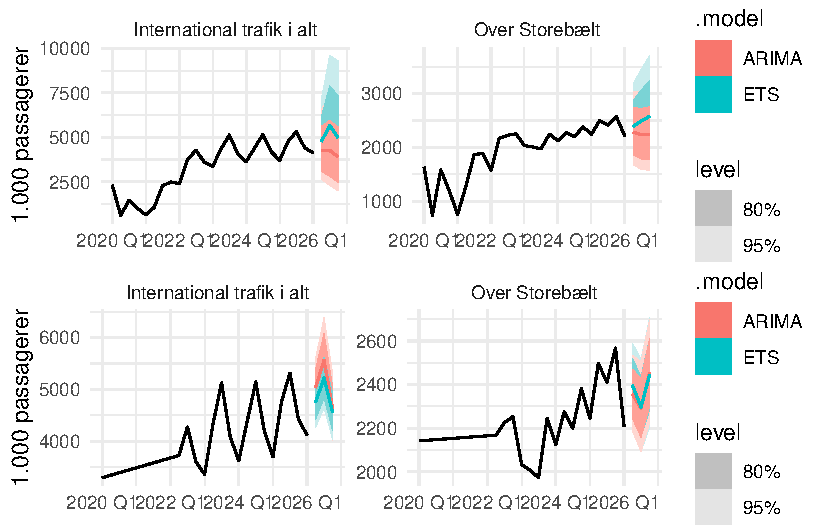
\includegraphics[keepaspectratio]{forecast_files/figure-pdf/fig-forecast-1.pdf}}

}

\caption{\label{fig-forecast}Forecast med prædiktionsintervaller (80\%
og 95\%)}

\end{figure}%

Forecasts er baseret på modeller estimeret på det fulde datasæt
(2006Q1-2026Q1) med en horisont på fire kvartaler til 2027Q1. Log
transformationen medfører assymetriske prædiktionsintervaller på
originalskalaen (log normal fordeling) hvor opadrettede intervaller er
bredere end nedadrettede. Intervallerne udvides med horisonten i takt
med akkummuleret usikkerhed.

ARIMA \& ETS er enige om retningen for begge serier, fortsat positiv
vækst for international trafik i forlængelse af genopretningstrenden fra
2022 og mere stabil, moderat vækst for storeblælt konsistent med lavere
trendstyrke. For international trafik er 80\% \& 95\%
prædiktionsintervallerne brede, konsistent med den højere
modelusikkerhed afspejlet i ljung-box resultaterne.

\section{Sammenfatning og konklusion}\label{sammenfatning-og-konklusion}

\begin{Shaded}
\begin{Highlighting}[]
\NormalTok{stl\_features }\OtherTok{\textless{}{-}} \FunctionTok{bind\_rows}\NormalTok{(}
\NormalTok{  jernbanedata        }\SpecialCharTok{\%\textgreater{}\%} \FunctionTok{features}\NormalTok{(x1000\_passagerer, feat\_stl) }\SpecialCharTok{\%\textgreater{}\%} \FunctionTok{mutate}\NormalTok{(}\AttributeTok{data =} \StringTok{"Inkl. corona"}\NormalTok{),}
\NormalTok{  jernbanedata\_corona }\SpecialCharTok{\%\textgreater{}\%} \FunctionTok{features}\NormalTok{(x1000\_passagerer, feat\_stl) }\SpecialCharTok{\%\textgreater{}\%} \FunctionTok{mutate}\NormalTok{(}\AttributeTok{data =} \StringTok{"Uden corona"}\NormalTok{)}
\NormalTok{) }\SpecialCharTok{\%\textgreater{}\%}
  \FunctionTok{select}\NormalTok{(key, data, trend\_strength, seasonal\_strength\_year)}
\end{Highlighting}
\end{Shaded}

\begin{Shaded}
\begin{Highlighting}[]
\NormalTok{bedste }\OtherTok{\textless{}{-}}\NormalTok{ resultat }\SpecialCharTok{\%\textgreater{}\%}
  \FunctionTok{filter}\NormalTok{(.type }\SpecialCharTok{==} \StringTok{"Test"}\NormalTok{) }\SpecialCharTok{\%\textgreater{}\%}
  \FunctionTok{group\_by}\NormalTok{(data, key) }\SpecialCharTok{\%\textgreater{}\%}
  \FunctionTok{slice\_min}\NormalTok{(RMSE, }\AttributeTok{n =} \DecValTok{1}\NormalTok{) }\SpecialCharTok{\%\textgreater{}\%}
  \FunctionTok{select}\NormalTok{(key, data, }\AttributeTok{Bedste\_model =}\NormalTok{ .model, MASE, RMSE)}
\end{Highlighting}
\end{Shaded}

\begin{Shaded}
\begin{Highlighting}[]
\NormalTok{sammenfatning }\OtherTok{\textless{}{-}}\NormalTok{ stl\_features }\SpecialCharTok{\%\textgreater{}\%}
  \FunctionTok{left\_join}\NormalTok{(bedste, }\AttributeTok{by =} \FunctionTok{c}\NormalTok{(}\StringTok{"key"}\NormalTok{, }\StringTok{"data"}\NormalTok{)) }\SpecialCharTok{\%\textgreater{}\%}
  \FunctionTok{mutate}\NormalTok{(}
    \AttributeTok{COVID\_impact =} \FunctionTok{case\_when}\NormalTok{(}
\NormalTok{      data }\SpecialCharTok{==} \StringTok{"Inkl. corona"} \SpecialCharTok{\textasciitilde{}} \StringTok{"Ja – ubehandlet"}\NormalTok{,}
\NormalTok{      data }\SpecialCharTok{==} \StringTok{"Uden corona"}  \SpecialCharTok{\textasciitilde{}} \StringTok{"Interpoleret"}
\NormalTok{    )}
\NormalTok{  ) }\SpecialCharTok{\%\textgreater{}\%}
  \FunctionTok{select}\NormalTok{(}
    \AttributeTok{Serie        =}\NormalTok{ key,}
\NormalTok{    datasæt      }\OtherTok{=}\NormalTok{ data,}
    \AttributeTok{Trend        =}\NormalTok{ trend\_strength,}
\NormalTok{    Sæson        }\OtherTok{=}\NormalTok{ seasonal\_strength\_year,}
    \AttributeTok{COVID        =}\NormalTok{ COVID\_impact,}
\NormalTok{    Bedste\_model,}
\NormalTok{    RMSE}
\NormalTok{  ) }\SpecialCharTok{\%\textgreater{}\%}
  \FunctionTok{arrange}\NormalTok{(Serie, datasæt)}

\NormalTok{sammenfatning }\SpecialCharTok{\%\textgreater{}\%}
  \FunctionTok{kbl}\NormalTok{(}\AttributeTok{digits =} \DecValTok{2}\NormalTok{, }\AttributeTok{booktabs =} \ConstantTok{TRUE}\NormalTok{) }\SpecialCharTok{\%\textgreater{}\%}
  \FunctionTok{kable\_styling}\NormalTok{(}\AttributeTok{latex\_options =} \FunctionTok{c}\NormalTok{(}\StringTok{"striped"}\NormalTok{, }\StringTok{"hold\_position"}\NormalTok{))}
\end{Highlighting}
\end{Shaded}

\begin{table}

\caption{\label{tbl-sammenfatning}Sammenfatningsoversigt: Nøgletal per
serie og datasæt}

\centering{

\centering
\begin{tabular}[t]{llrrllr}
\toprule
Serie & datasæt & Trend & Sæson & COVID & Bedste\_model & RMSE\\
\midrule
\cellcolor{gray!10}{International trafik i alt} & \cellcolor{gray!10}{Inkl. corona} & \cellcolor{gray!10}{0,97} & \cellcolor{gray!10}{0,81} & \cellcolor{gray!10}{Ja – ubehandlet} & \cellcolor{gray!10}{Auto} & \cellcolor{gray!10}{215,82}\\
International trafik i alt & Uden corona & 0,96 & 0,86 & Interpoleret & M3 & 94,73\\
\cellcolor{gray!10}{Over Storebælt} & \cellcolor{gray!10}{Inkl. corona} & \cellcolor{gray!10}{0,87} & \cellcolor{gray!10}{0,51} & \cellcolor{gray!10}{Ja – ubehandlet} & \cellcolor{gray!10}{M2} & \cellcolor{gray!10}{69,55}\\
Over Storebælt & Uden corona & 0,91 & 0,80 & Interpoleret & M2 & 121,27\\
\bottomrule
\end{tabular}

}

\end{table}%

Seriekarakteristika: Begge serier har stærke trendkomponenter
(0,87-0,97). International trafik har den stærkeste sæsonstruktur (0,86
uden corona). Storebælt er mere afdæmpet sæsonstruktur (0,80) som
forstyrres uforholdsmæssigt af corona. Guerrero analysen (lambda = 0 på
coronafri data) understøtter log transformation gennemgående.

Stationaritet: Coronaperioden svækker stationaritetsvurderingen. KPSS
afviser ikke stationaritet inkl. corona. og auto ARIMA vælger d=D=0. Det
interpolerede datasæt giver et mere korrekt grundlag, hvor D=1 vælges
konsistent med den underliggende sæsontrend.

Modelpræstation: ETS opnår den laveste AICc \& TSCV RMSE for
international trafik inkl. corona (762) mod ARIMA (845). For storebælt
uden corona (RMSE=120, MASE=1,14). Den exhaustive ARIMA søgning
forbedrer AICc betydeligt, særligt for international trafik inkl. corona
(5,4 til -4,8)

Residualanalyse: International trafik udviser vedvarende autokorrelerede
residualer i begge modelklasser, og datasæt (Ljung-Box p \textless{}
0,05), hvilket antyder en dynamik uden for ARIMA/ETS rammens rækkevidde.
Storebælt uden corona er den eneste kombination, hvor begge modeltypers
residualtests består testen.

Benchmark og begrænsninger: Ingen af modellerne opnår MASE \textless{} 1
i TSCV, ingen slår SNAIVE. Inkl corona skyldes dette corona kvartaler
som historiske mønstre ikke kan forudsige. Uden corona er MASE tæt på,
men over 1. Corona interpolationen er analysens primære metodologiske
forbehold, da interpolerede observationer er et skøn, og resultater på
det rensede datasæt skal tolkes derefter.

\newpage

\subsection{Bilag}\label{bilag}

\appendix

\section*{Bilag A: Stationaritetstest}\label{sec-bilag-a}
\addcontentsline{toc}{section}{Bilag A: Stationaritetstest}

\begin{table}

\caption{\label{tbl-kpss-bilag}}

\centering{

\centering
\caption{\label{tab:tbl-kpss-bilag}KPSS-test — H0: stationær}
\centering
\begin{tabular}[t]{lrr}
\toprule
key & kpss\_stat & kpss\_pvalue\\
\midrule
\cellcolor{gray!10}{International trafik i alt} & \cellcolor{gray!10}{0,1865} & \cellcolor{gray!10}{0,1}\\
Over Storebælt & 0,2156 & 0,1\\
\bottomrule
\end{tabular}

\centering
\caption{\label{tab:tbl-kpss-bilag}Anbefalet antal sæsondifferentieringer (D)}
\centering
\begin{tabular}[t]{lr}
\toprule
key & nsdiffs\\
\midrule
\cellcolor{gray!10}{International trafik i alt} & \cellcolor{gray!10}{0}\\
Over Storebælt & 0\\
\bottomrule
\end{tabular}

\centering
\caption{\label{tab:tbl-kpss-bilag}Anbefalet antal ordinære differentieringer (d)}
\centering
\begin{tabular}[t]{lr}
\toprule
key & ndiffs\\
\midrule
\cellcolor{gray!10}{International trafik i alt} & \cellcolor{gray!10}{0}\\
Over Storebælt & 0\\
\bottomrule
\end{tabular}

\centering
\caption{\label{tab:tbl-kpss-bilag}Anbefalet d efter sæsondifferentiering (D=1)}
\centering
\begin{tabular}[t]{lr}
\toprule
key & ndiffs\\
\midrule
\cellcolor{gray!10}{International trafik i alt} & \cellcolor{gray!10}{0}\\
Over Storebælt & 0\\
\bottomrule
\end{tabular}

}

\end{table}%

\section*{Bilag B: SNAIVE benchmark}\label{sec-bilag-b}
\addcontentsline{toc}{section}{Bilag B: SNAIVE benchmark}

\begin{table}[!h]
\centering
\caption{\label{tab:benchmark-bilag}SNAIVE benchmark – Inkl. corona}
\centering
\begin{tabular}[t]{lllrrrrrrrr}
\toprule
.model & key & .type & ME & RMSE & MAE & MPE & MAPE & MASE & RMSSE & ACF1\\
\midrule
\cellcolor{gray!10}{SNAIVE(log(x1000\_passagerer))} & \cellcolor{gray!10}{International trafik i alt} & \cellcolor{gray!10}{Test} & \cellcolor{gray!10}{3,68} & \cellcolor{gray!10}{929,59} & \cellcolor{gray!10}{532,93} & \cellcolor{gray!10}{-16,92} & \cellcolor{gray!10}{34,73} & \cellcolor{gray!10}{1,26} & \cellcolor{gray!10}{1,21} & \cellcolor{gray!10}{0,82}\\
SNAIVE(log(x1000\_passagerer)) & Over Storebælt & Test & 0,65 & 360,41 & 236,66 & -4,03 & 16,46 & 1,37 & 1,23 & 0,60\\
\bottomrule
\end{tabular}
\end{table}

\begin{table}[!h]
\centering
\caption{\label{tab:benchmark-bilag}SNAIVE benchmark – Uden corona}
\centering
\begin{tabular}[t]{lllrrrrrrrr}
\toprule
.model & key & .type & ME & RMSE & MAE & MPE & MAPE & MASE & RMSSE & ACF1\\
\midrule
\cellcolor{gray!10}{SNAIVE(log(x1000\_passagerer))} & \cellcolor{gray!10}{International trafik i alt} & \cellcolor{gray!10}{Test} & \cellcolor{gray!10}{117,16} & \cellcolor{gray!10}{259,98} & \cellcolor{gray!10}{191,78} & \cellcolor{gray!10}{2,80} & \cellcolor{gray!10}{5,09} & \cellcolor{gray!10}{1,01} & \cellcolor{gray!10}{1,03} & \cellcolor{gray!10}{0,34}\\
SNAIVE(log(x1000\_passagerer)) & Over Storebælt & Test & 18,52 & 128,76 & 100,65 & 0,61 & 4,73 & 1,21 & 1,18 & 0,66\\
\bottomrule
\end{tabular}
\end{table}

\section*{Bilag C: Ljung-Box tests}\label{sec-bilag-c}
\addcontentsline{toc}{section}{Bilag C: Ljung-Box tests}

\begin{verbatim}
\begin{table}[!h]
\centering
\caption{\label{tab:ljung-bilag}Ljung-Box ETS – International trafik i alt – Inkl. corona}
\centering
\begin{tabular}[t]{llrr}
\toprule
key & .model & lb\_stat & lb\_pvalue\\
\midrule
\cellcolor{gray!10}{International trafik i alt} & \cellcolor{gray!10}{Auto} & \cellcolor{gray!10}{17,16} & \cellcolor{gray!10}{0,03}\\
\bottomrule
\end{tabular}
\end{table}


\begin{table}[!h]
\centering
\caption{\label{tab:ljung-bilag}Ljung-Box ETS – Over Storebælt – Inkl. corona}
\centering
\begin{tabular}[t]{llrr}
\toprule
key & .model & lb\_stat & lb\_pvalue\\
\midrule
\cellcolor{gray!10}{Over Storebælt} & \cellcolor{gray!10}{Auto} & \cellcolor{gray!10}{23,84} & \cellcolor{gray!10}{0}\\
\bottomrule
\end{tabular}
\end{table}
\end{verbatim}

\begin{verbatim}
\begin{table}[!h]
\centering
\caption{\label{tab:ljung-bilag}Ljung-Box ETS – International trafik i alt – Uden corona}
\centering
\begin{tabular}[t]{llrr}
\toprule
key & .model & lb\_stat & lb\_pvalue\\
\midrule
\cellcolor{gray!10}{International trafik i alt} & \cellcolor{gray!10}{Auto} & \cellcolor{gray!10}{22,99} & \cellcolor{gray!10}{0}\\
\bottomrule
\end{tabular}
\end{table}


\begin{table}[!h]
\centering
\caption{\label{tab:ljung-bilag}Ljung-Box ETS – Over Storebælt – Uden corona}
\centering
\begin{tabular}[t]{llrr}
\toprule
key & .model & lb\_stat & lb\_pvalue\\
\midrule
\cellcolor{gray!10}{Over Storebælt} & \cellcolor{gray!10}{Auto} & \cellcolor{gray!10}{9,34} & \cellcolor{gray!10}{0,31}\\
\bottomrule
\end{tabular}
\end{table}
\end{verbatim}

\begin{verbatim}
\begin{table}[!h]
\centering
\caption{\label{tab:ljung-bilag}Ljung-Box ARIMA – International trafik i alt – Inkl. corona}
\centering
\begin{tabular}[t]{llrr}
\toprule
key & .model & lb\_stat & lb\_pvalue\\
\midrule
\cellcolor{gray!10}{International trafik i alt} & \cellcolor{gray!10}{Auto} & \cellcolor{gray!10}{12,61} & \cellcolor{gray!10}{0,03}\\
\bottomrule
\end{tabular}
\end{table}


\begin{table}[!h]
\centering
\caption{\label{tab:ljung-bilag}Ljung-Box ARIMA – Over Storebælt – Inkl. corona}
\centering
\begin{tabular}[t]{llrr}
\toprule
key & .model & lb\_stat & lb\_pvalue\\
\midrule
\cellcolor{gray!10}{Over Storebælt} & \cellcolor{gray!10}{Auto} & \cellcolor{gray!10}{10,96} & \cellcolor{gray!10}{0,05}\\
\bottomrule
\end{tabular}
\end{table}
\end{verbatim}

\begin{verbatim}
\begin{table}[!h]
\centering
\caption{\label{tab:ljung-bilag}Ljung-Box ARIMA – International trafik i alt – Uden corona}
\centering
\begin{tabular}[t]{llrr}
\toprule
key & .model & lb\_stat & lb\_pvalue\\
\midrule
\cellcolor{gray!10}{International trafik i alt} & \cellcolor{gray!10}{Auto} & \cellcolor{gray!10}{16,99} & \cellcolor{gray!10}{0,01}\\
\bottomrule
\end{tabular}
\end{table}


\begin{table}[!h]
\centering
\caption{\label{tab:ljung-bilag}Ljung-Box ARIMA – Over Storebælt – Uden corona}
\centering
\begin{tabular}[t]{llrr}
\toprule
key & .model & lb\_stat & lb\_pvalue\\
\midrule
\cellcolor{gray!10}{Over Storebælt} & \cellcolor{gray!10}{Auto} & \cellcolor{gray!10}{5,12} & \cellcolor{gray!10}{0,4}\\
\bottomrule
\end{tabular}
\end{table}
\end{verbatim}




\end{document}
